%% LaTeX2e class for student theses
%% sections/evaluation.tex
%% 
%% Karlsruhe Institute of Technology
%% Institute for Program Structures and Data Organization
%% Chair for Software Design and Quality (SDQ)
%%
%% Dr.-Ing. Erik Burger
%% burger@kit.edu
%%
%% Version 1.3.3, 2018-04-17

\chapter{Modellierung}
\label{ch:modellierung}
Wie bereits in \autoref{sec:eventbasetransformation} beschrieben bietet das PCM die Möglichkeit eventbasierte Kommunikation zu modellieren und auch eine konkrete MOM Architektur zu modellieren, die mithilfe einer Modelltransformation in die Systemarchitektur eingewoben wird. Diese Modellierung hat jedoch das Problem, dass die Kommunikation nur in eine Richtung funktioniert, wie in \autoref{img:oldEventBased}a zu sehen. Ein Sender sendet eine Nachricht an einen Empfänger und auf dem Weg dorthin durchläuft die Nachricht eine Komponentenkette und wird mit bestimmten Ressourcenanforderungen belegt. Der Empfänger erhält schließlich die Nachricht. In diesem Szenario fehlt jedoch die Warteschlange, die eine wichtige Komponente einer MOM ist. Eigentlich sollte die Komunikation wie in \autoref{img:oldEventBased}b abgebildet stattfinden. Der Sender sendet die Nachricht an die MOM, diese leitet die Nachricht an die entsprechende Warteschlange weiter und ein Empfänger holt sich die Nachricht ab, sobald er die Ressourcen dazu hat. Dieses Szenario ist mit der aktuellen eventbasierten Kommunikation in PCM nicht darstellbar, weil kein abholen einer Nachricht vorgesehen ist. Deshalb soll im Folgenden eine Modellierung präsentiert werden, die eine explizite Warteschlange und ein Verteilsystem, das Nachrichten an passenden Warteschlangen verteilt, modelliert.\par
Dazu soll zunächst mithilfe einer Anforderungserhebung in \autoref{sec:anforderungserhebung} Anforderungen gesammelt werden, die eine solche Modellierung erfüllen soll. Im Anschluss wird in \autoref{sec:modell} die Modellierung einer MOM vorgestellt, die die Anforderungen erfüllen soll. In \autoref{sec:modellkalibrierung} soll das Modell mithilfe der in \autoref{sec:rmqBenchmark} ausgemessenen MOM RMQ kalibriert werden. Dabei soll ein kalibrierter MOM Baustein entstehen, der sich wie die ausgemessene MOM verhalten soll. Schließlich wird in \autoref{sec:momsimulation} das MOM Modell in mehreren Simulationen eingesetzt werden und mit den realem Messungen verglichen. 
\begin{figure}
\center
  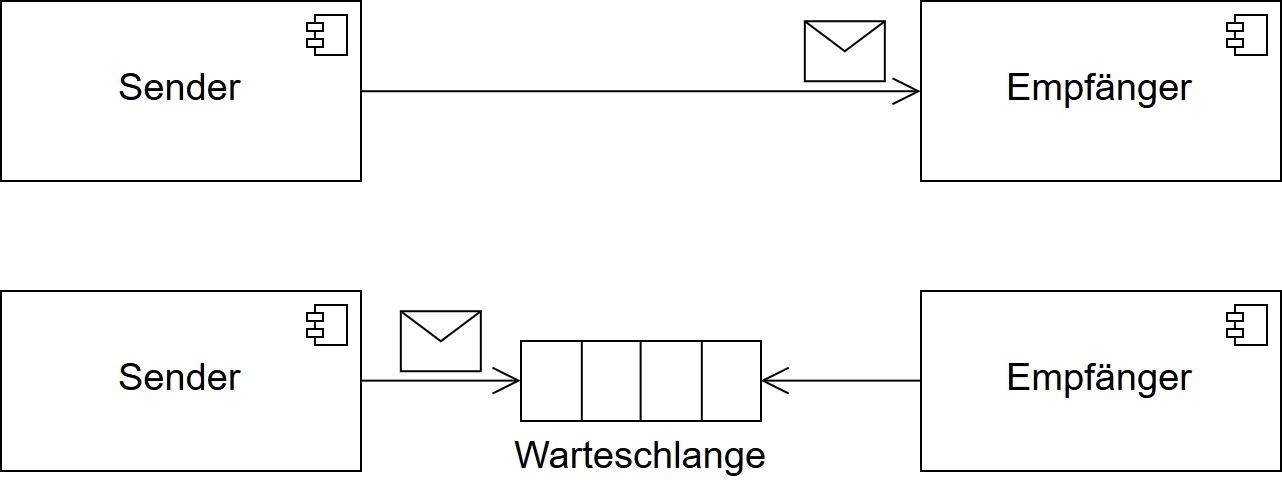
\includegraphics[width=1\textwidth]{images/modelling/oldEventBased.png}
  \caption{Aktuelle eventbasierte Kommunikation}
  \label{img:oldEventBased}
\end{figure}


\section{Anforderungserhebung}
\label{sec:anforderungserhebung}
Aus der Definition einer MOM (siehe Grundlagen) und den Messungen aus \autoref{ch:mom} wurden die folgenden Anforderungen an eine Modellierung abgeleitet. Dabei wurde unterschieden zwischen technischen Anforderungen, also was die Modellierung leisten muss und Anforderungen an die Nutzbarkeit unterschieden. 
Zu den technischen Anforderungen gehören:
\begin{itemize}
    \item Die Modellierung soll das allgemeine Verhalten einer MOM abbilden können.
    \item Asynchrones senden und empfangen von Nachrichten.
    \item Es soll möglich sein eine Nachricht an eine bestimmte Warteschlange oder Topic senden zu können.
    \item Der Füllstand der Warteschlange soll mithilfe der Performanzanalyse ermittelt werden können.
    \item Die Latenz einer Nachricht soll mithilfe der Performanzanalyse ermittelt werden können.
\end{itemize}
Der Benutzer der Modellierung muss in der Lage sein die Folgenden Dinge angeben zu können:
\begin{itemize}
    \item Die Nachrichtengröße muss definierbar sein
    \item Die Topic einer Nachricht muss definierbar sein
    \item Die Anzahl der Nachrichten die pro Sekunde gesendet werden muss angegeben werde können
\end{itemize}

%Angabe des Durchsatzes \\


%Das Ziel ist es eine allgemeine MOM Modellierung zu erstellen, die das Verhalten einer MOM abbilden kann. Dabei soll nicht Wert auf ein spezielles Verhalten gelegt werden. Stattdessen soll es moeglich sein die Modellierung um Konfigurationen, wie zum Beispiel RMQs lazy Queues, erweitern zu koennen. 

\section{Modell}
Im Folgenden soll eine Modellierung einer MOM präsentiert werden die die zuvor definierten Anforderungen erfüllt. Dabei war nicht das Ziel eine Meta-Modell Erweiterung zu erstellen, sondern mit bereits existierenden PCM-Elementen zu arbeiten. 

%Anhand der bekannten MOM Architekturen aus der Untersuchung verschiedener MOMs wurde versucht zu definieren wie eine MOM modelliert werden kann. Dabei wurden die Anforderungen versucht umzusetzen. \\
%- 2 Moeglichkeiten entweder mit oder ohne Exchange explizit zu modellieren.\\
%- Vorteil Explizit: RDs fuer verteilung (konnte aber nicht ausgemessen werden) \\
%- Nachrichten Typen mitschicken (fanout, direct) und in Branches auswerten

\subsection{Repository}
Das Repository wird vom Komponentenentwickler verwendet um neue Komponenten zu erstellen und vom Systemarchitekt um Komponenten zu entnehmen. ... \\
Die untersuchte MOM Architektur besteht aus einem Verteiler und einer Warteschlange. Deshalb wurdem die in \autoref{img:mom_repository} abgebildeten Komponenten und Schnittstellen definiert. Die Schnittstelle nach ausen soll die IExchange Schnittstelle sein. Diese bietet zwei Signaturen an. Eine zum Empfange (receive) und eine zum Senden (distribute) einer Nachricht. Beide Methoden werden von der Komponente Exchange angeboten. IQueue ist die zweite Schnittstelle. Diese bietet auch zwei Signaturen an. Eine um eine Nachricht in eine Warteschlange abzulegen (put) und eine weitere die eine Nachricht aus der Warteschlange entnimmt (get). Diese Schnittstelle wird von der Komponente Queue angeboten. Diese Komponenten, die eine Warteschlange abbildeen soll, besitzt eine Passive Resource die das Verhalten einer Warteschlange simulieren soll. Eine Passive Ressouce ist... (TODO). Dabei wird das ablegen in die Warteschlange als release auf die passive Ressource und das entnehmen aus der Warteschlange als aquire auf die passive Ressource modelliert. Die Exchange Komponente benötigt eine Komponente die die IQueue Schnittstelle anbietet. Die Idee ist, dass alle Warteschlangen die benötigt werden von der Exchange Komponente required werden. In \autoref{img:mom_repository} sind das aktuell zwei Warteschlange. Mithilfe des RDSEFFs kann die Exchange Komponente zwischen den Warteschlangen wechseln. Dies ist in \autoref{img:queueBranch} dargestellt. Dabei wird mithilfe eines GuardedBranch geprüft an welche Warteschlange die ankommenden Nachricht gehen soll. Der Fall, dass eine Nachricht aus der Warteschlange entnommen wird funktioniert genauso. 


%Dieser Ansatz ermöglicht es jedoch nicht einzelne Nachrichten durch das System zu verfolgen. \\


\begin{figure}
\center
  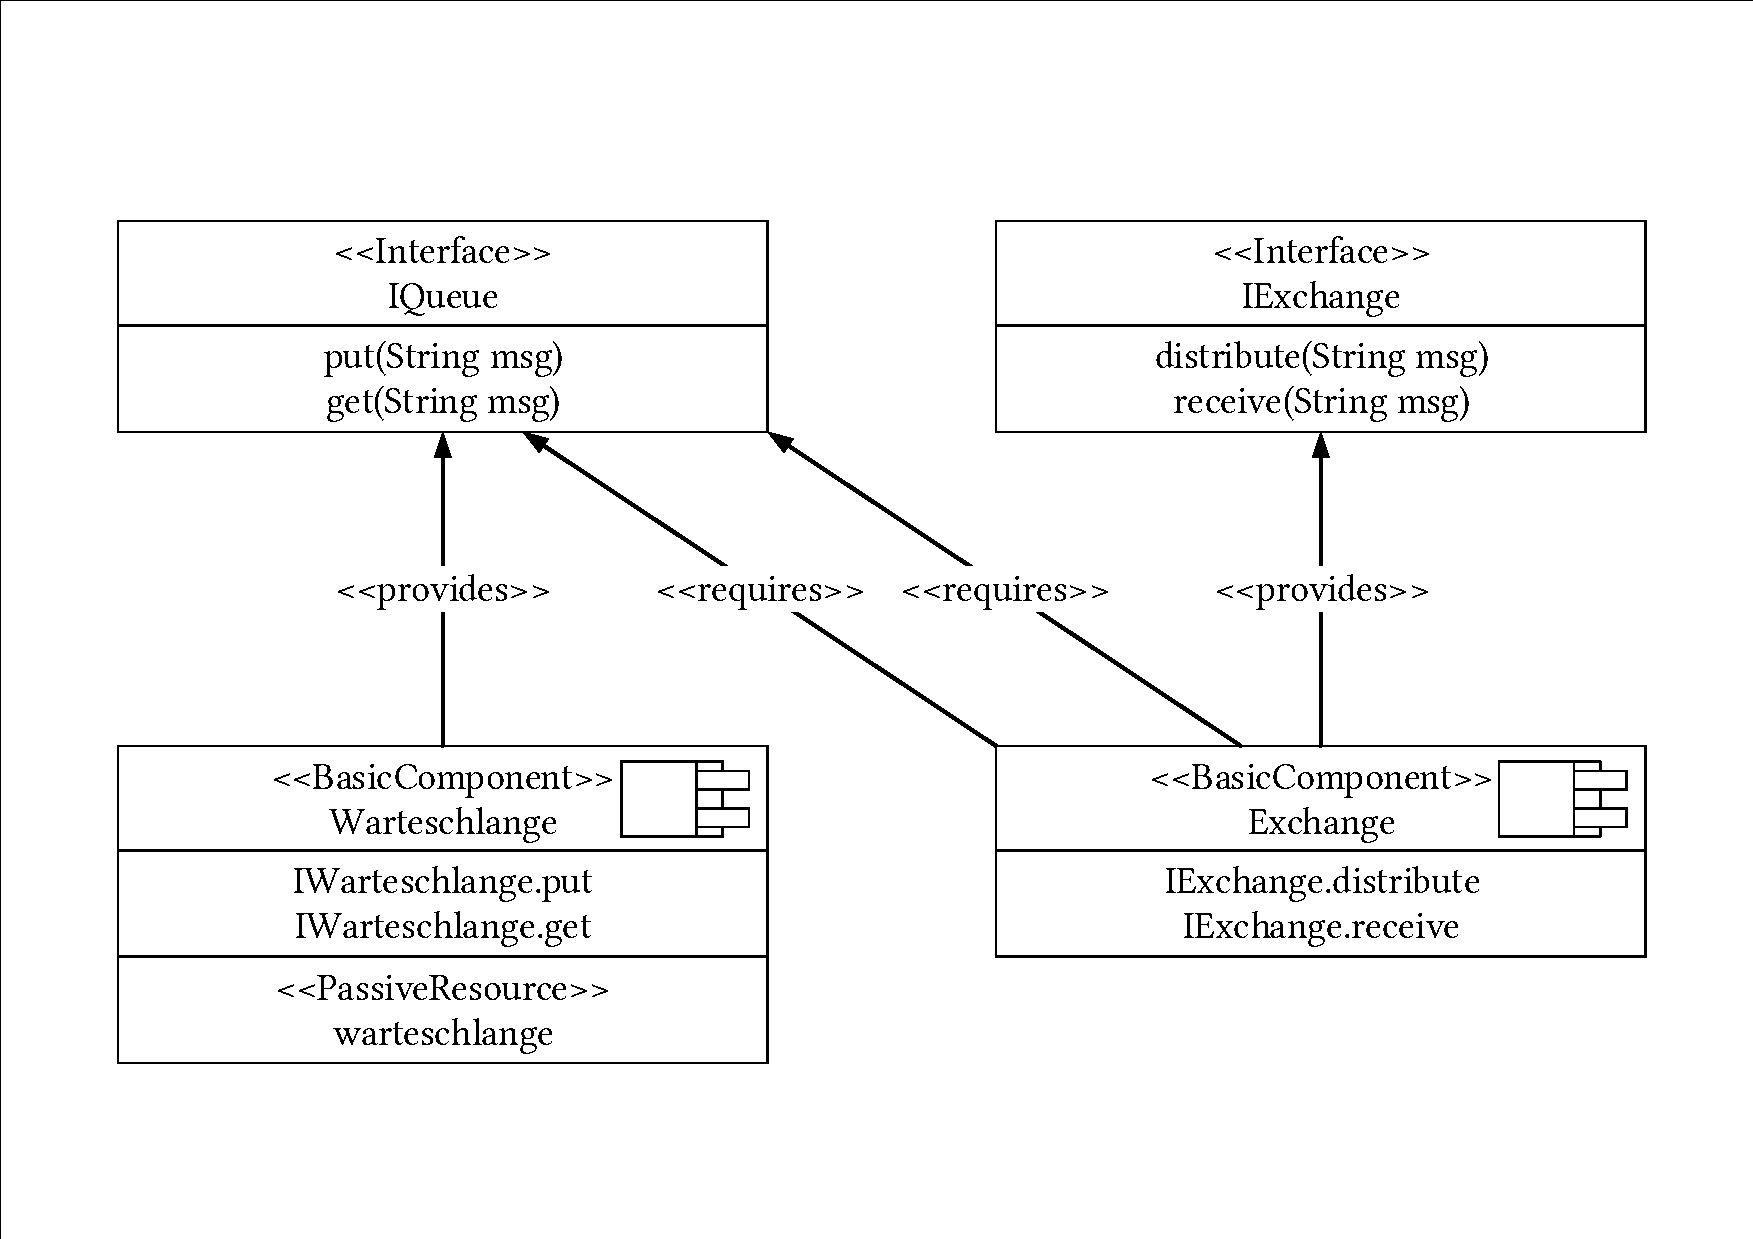
\includegraphics[width=1\textwidth]{images/modelling/repository.pdf}
  \caption{Repository einer MOM mit Exchange und Warteschlange}
  \label{img:mom_repository}
\end{figure}

\begin{figure}
\center
  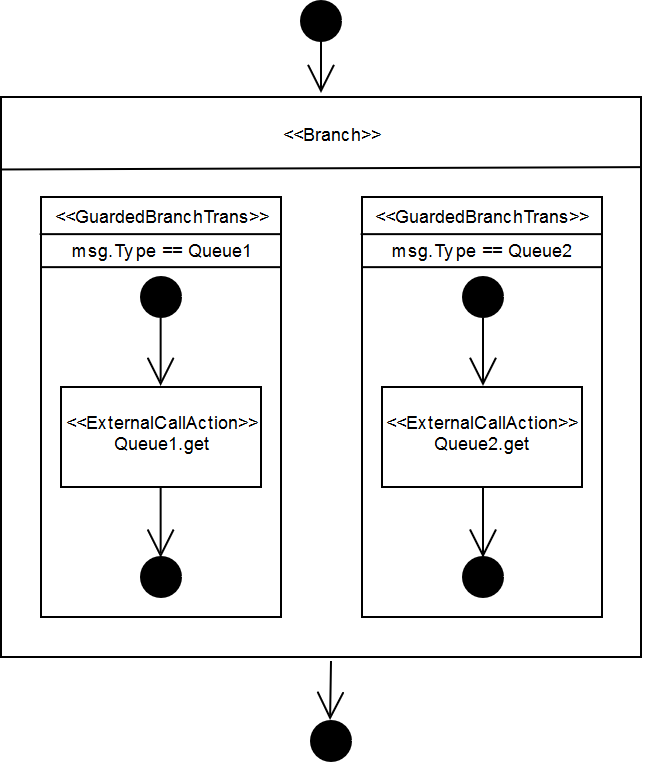
\includegraphics[width=0.7\textwidth]{images/modelling/branchSeff.png}
  \caption{Repository einer MOM mit Exchange und Warteschlange}
  \label{img:queueBranch}
\end{figure}

\subsection{System}
Im Systemmodell werden die einzelnen Komponenten aus dem Repository vom Softwarearchitekten zu einem System zusammengesetzt. Der Software-Architekt kann nun die Komponenten aus dem zuvor definierten Repository zusammensetzen. Dabei kann er zunächst entscheiden, wie viele Exchange Komponenten im System exisitieren sollen. Wie auch in RMQ kann eine MOM aus mehreren Exchanges bestehen, die sich auf unterschiedlichen Maschinen befinden können. An einen Exchange werden dann die dazugehörigen Warteschlangen angeschlossen. Da ein Exchange eine Schnittstell zum Senden und Empfangen von Nachrichten anbietet, können beliebig viele Sender und Empfänger Komponenten an einen Exchange angeschlossen werden. In \autoref{img:mom_system} ist ein Systemmodell mit zwei Exchange Komponenten abgebildet. Dabei hat Exchange1 zwei Warteschlangen Komponenten und Exchange2 nur eine Warteschlange angeschlossen. Außerdem sind an Exchange1 je ein Sender und Empfänger angeschlossen. An Exchange2 sind zwei Sender und ein Empfänger angeschlossen. 

\begin{figure}
\center
  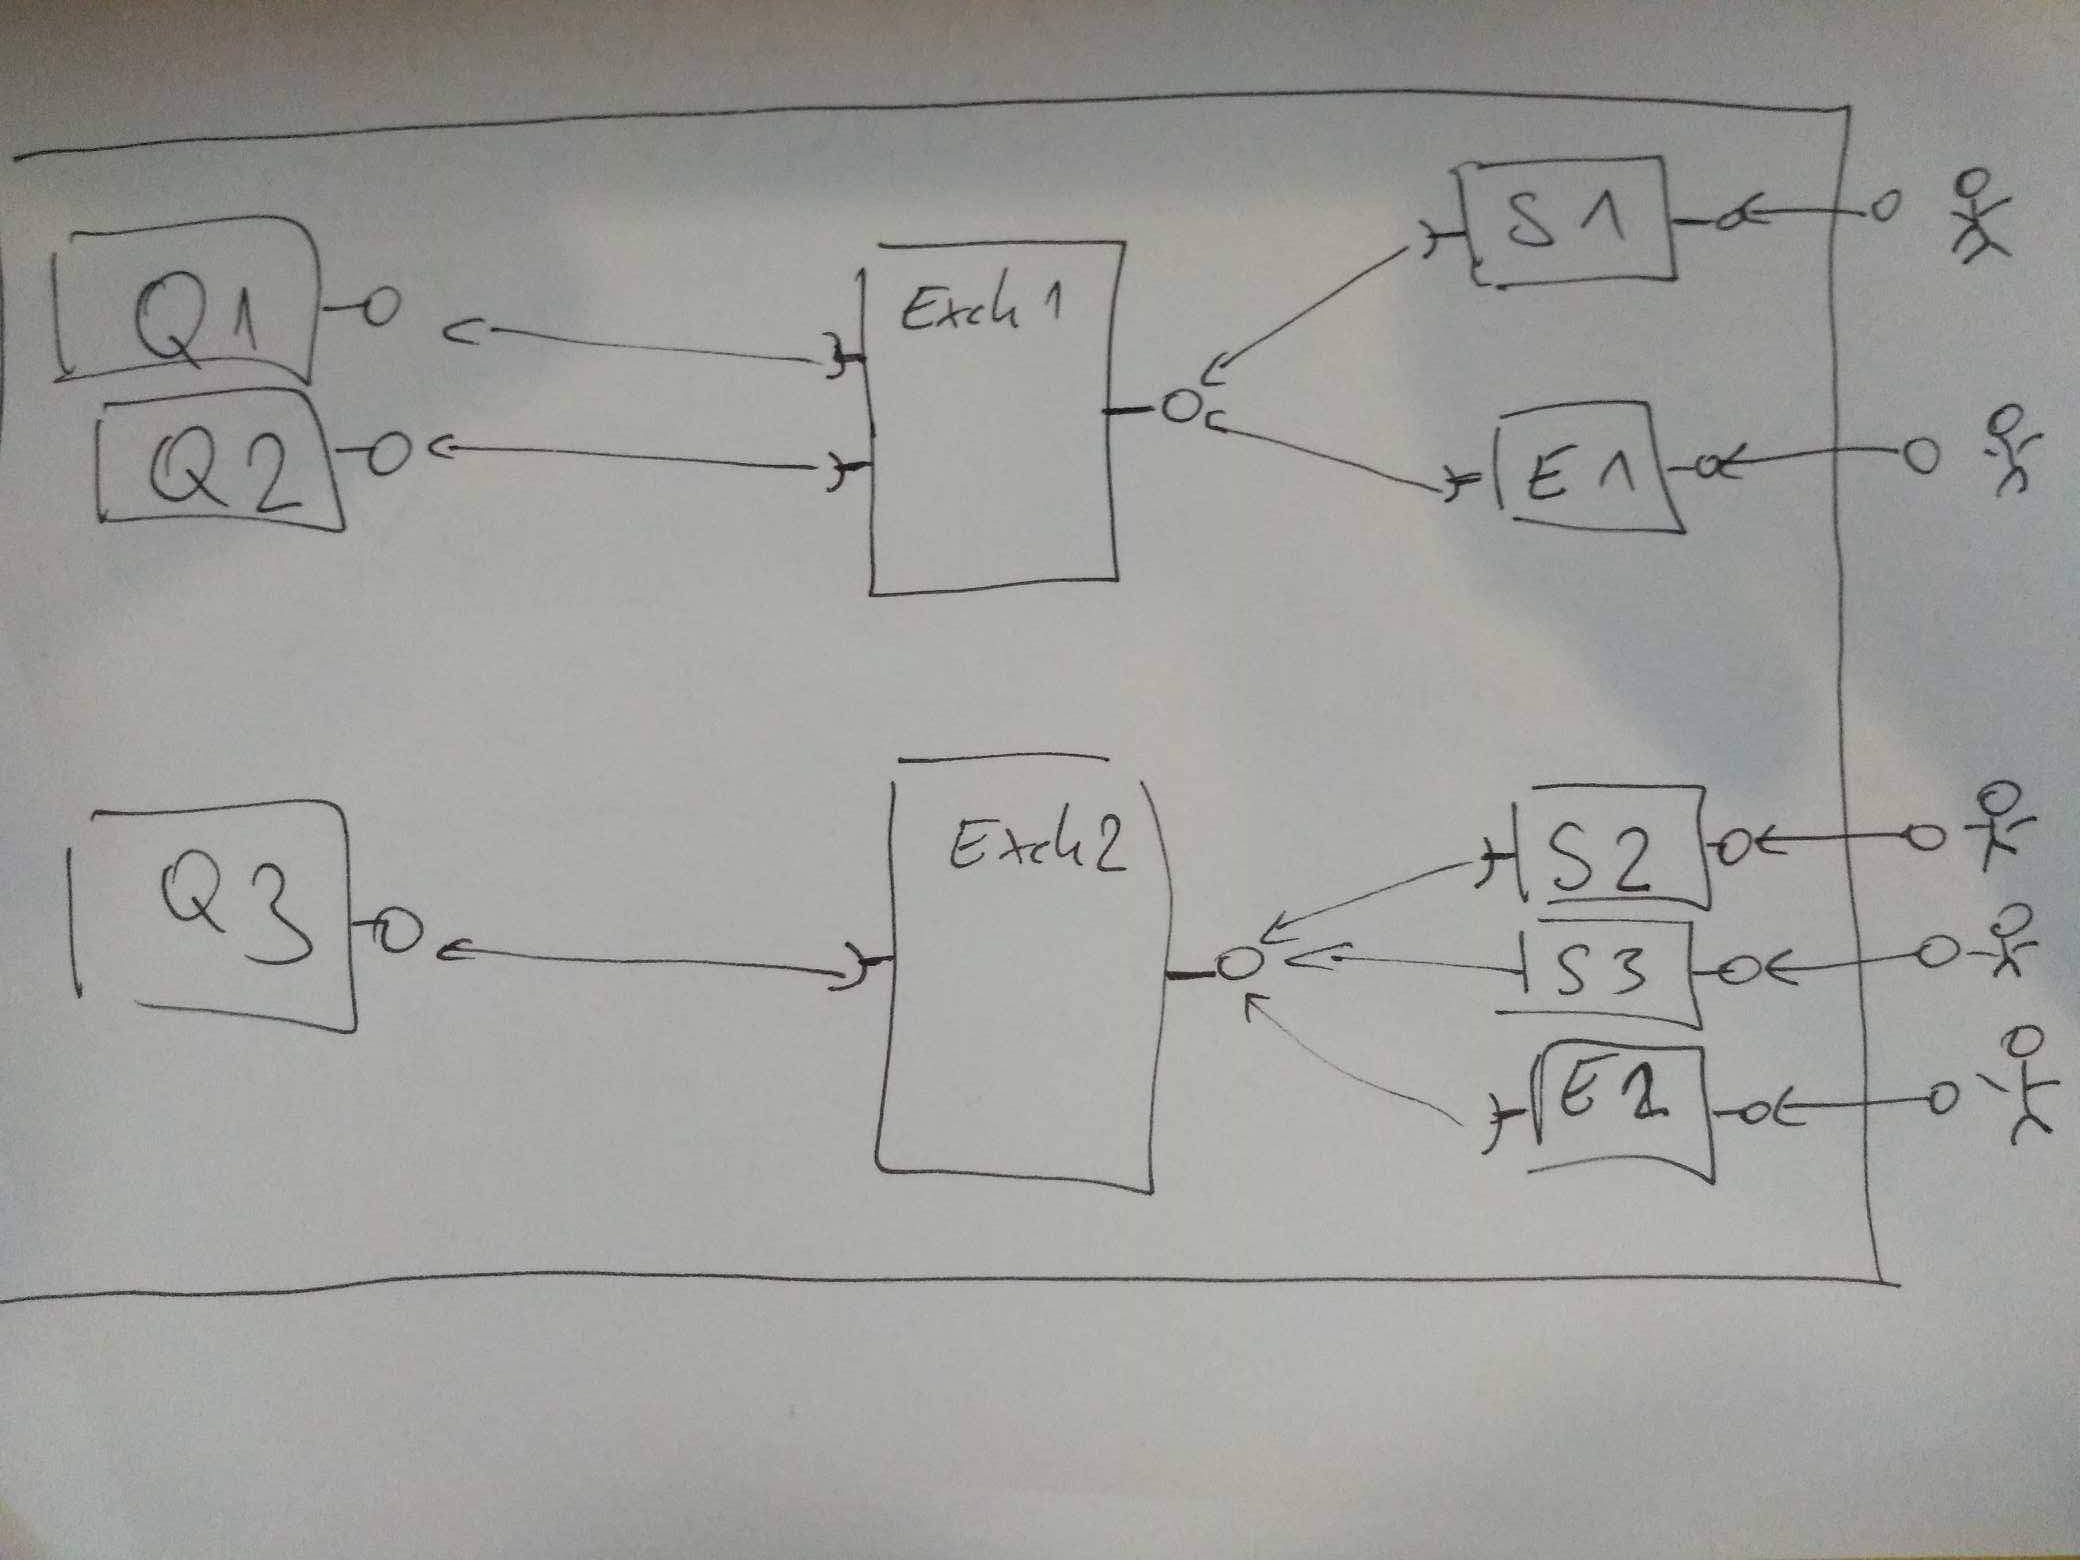
\includegraphics[width=1\textwidth]{images/modelling/system.png}
  \caption{Systemmodell einer MOM}
  \label{img:mom_system}
\end{figure}
\subsection{Ausführungsumgebung und Allokation}
Im Ausführungs-Umgebungs-Modell kann der Software-Verteilungs-Experte die Hardware Knoten und Netzwerkverbindungen darstellen. Für jeden Exchange und jede Warteschlange kann eine eigene Ressource definiert werden. Außerdem müssen die einzelnen Verbindungen zwischen einem Exchange und den Sendern und Empfängern modelliert werden. Falls Exchange und Warteschlange sich auf unterschiedlichen Ressourcen befinden, müssen die Verbindungen auch modelliert werden. In \autoref{img:mom_ressorceEnv} ist eine mögliche Ausführungsumgebung für das oben beschriebene System dargestellt. Die Ausführungsumgebung besteht aus je einer MOM Ressource für den jeweiligen Exchange und die an ihn angeschlossenen Warteschlangen. Die einzelnen Sender und Empfänger sind jeweils auf eigenen Ressourcen verteilt und sind über Netzwerkverbindungen mit der jeweiligen MOM Ressource verbungen. 
\begin{figure}
\center
  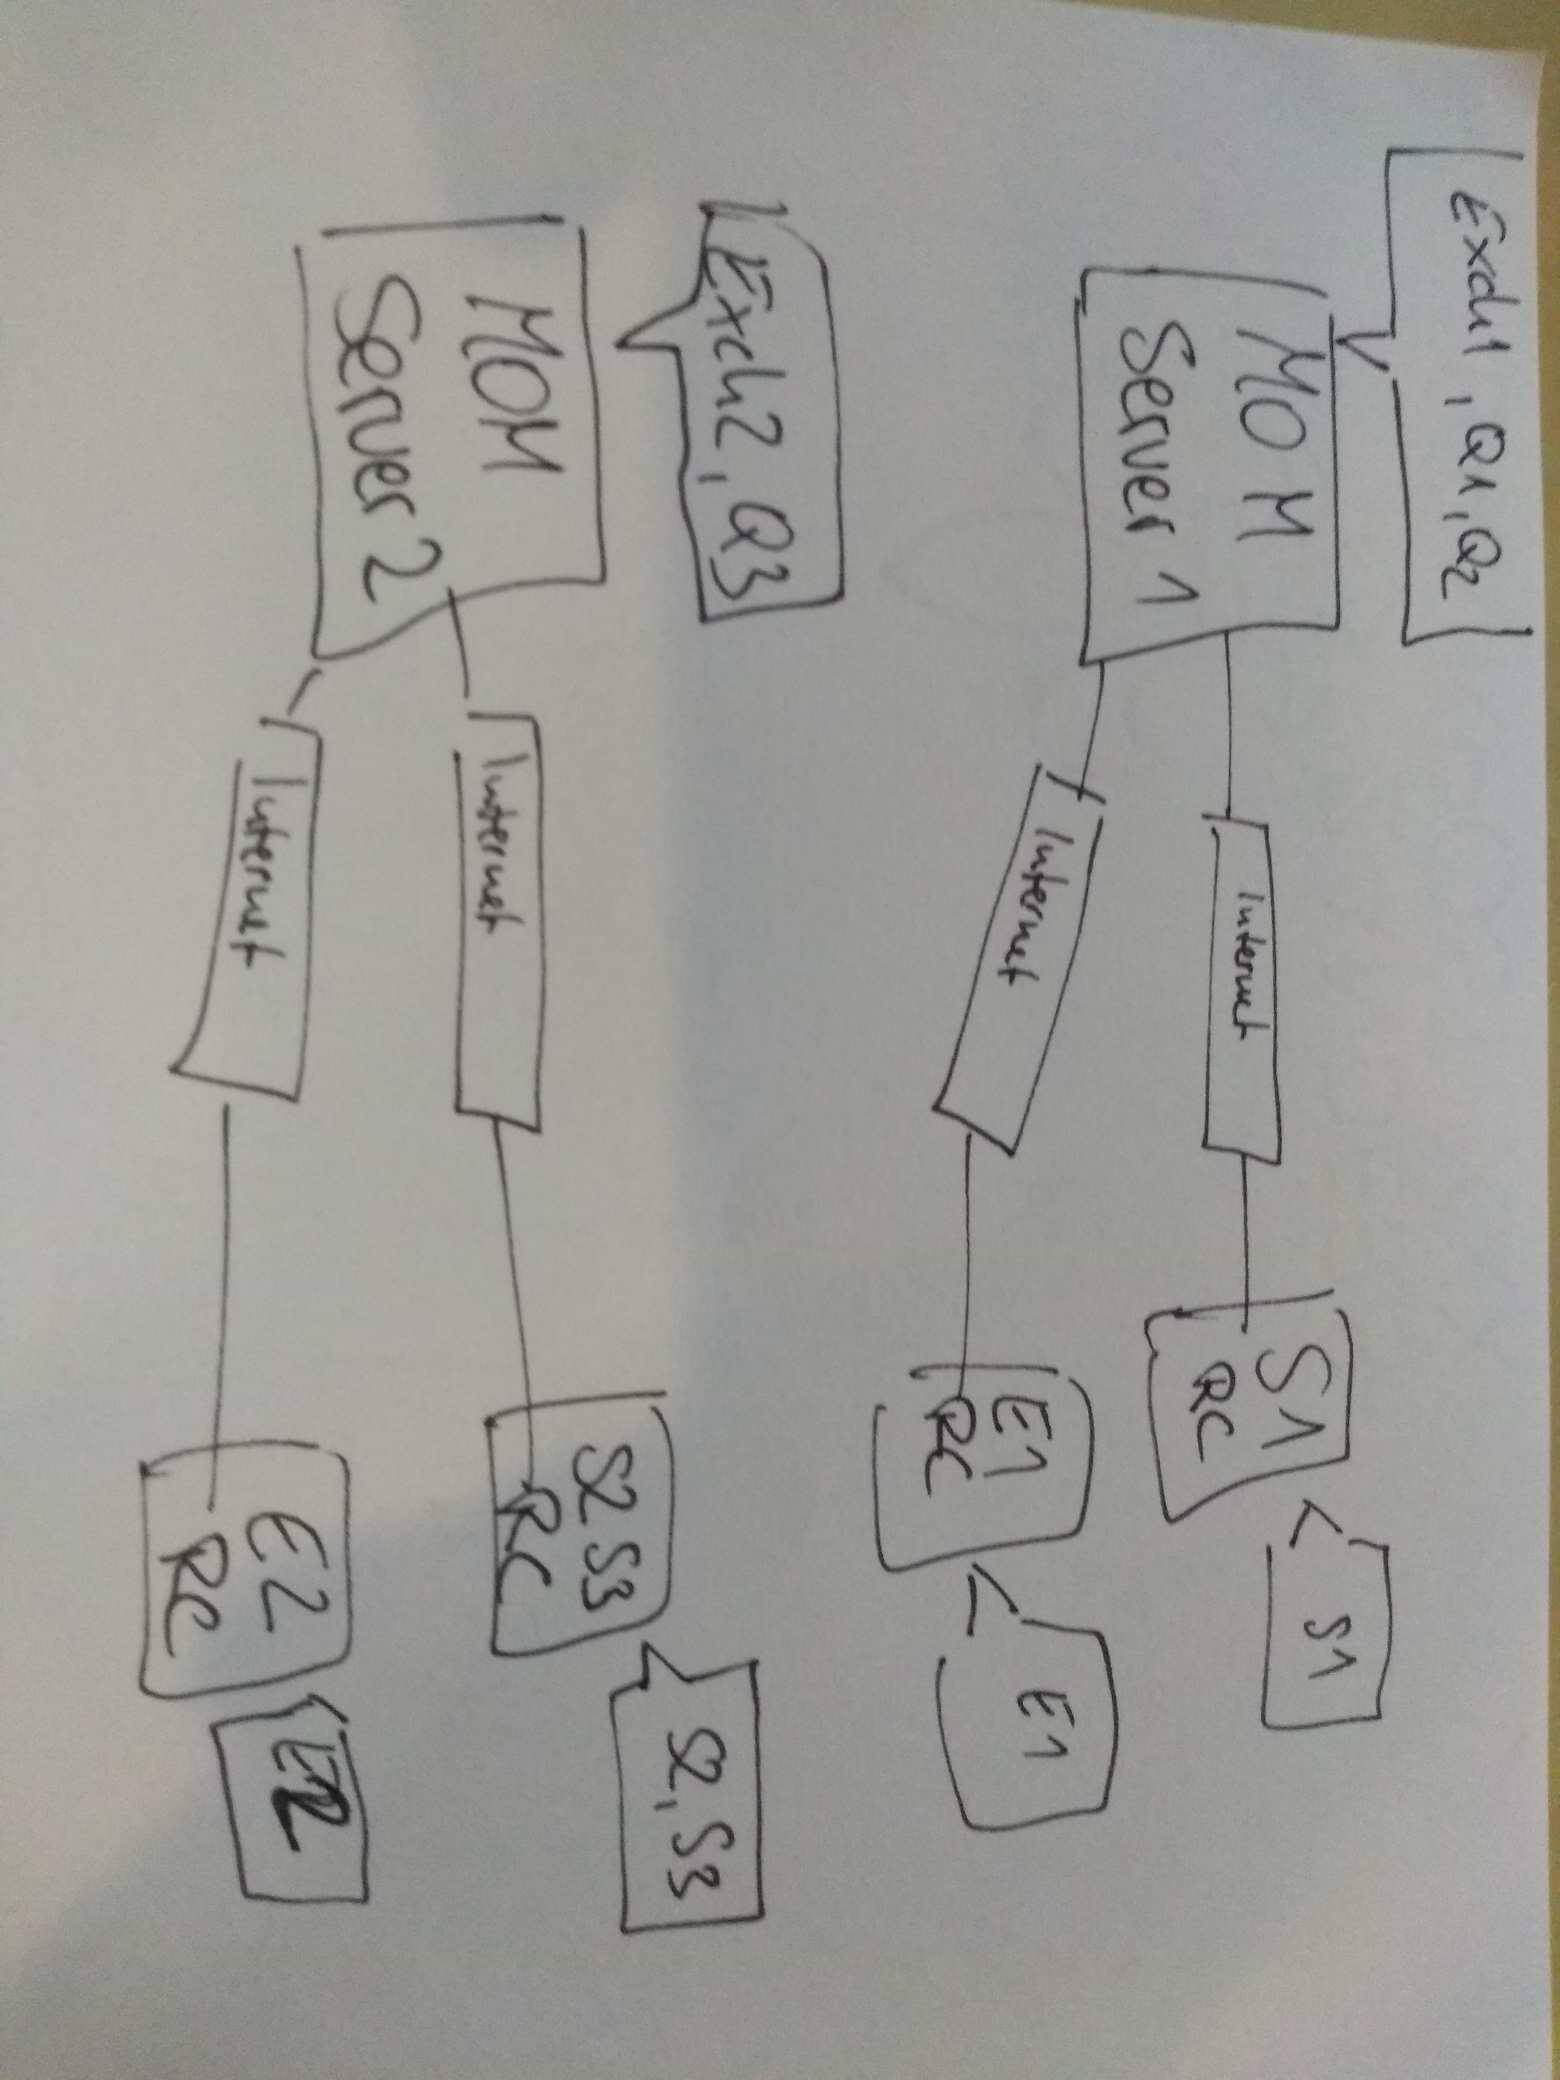
\includegraphics[width=1\textwidth]{images/modelling/recenv.png}
  \caption{Ausführungsumgebung und Allokation einer MOM}
  \label{img:mom_ressorceEnv}
\end{figure}

\subsection{Nutzungsmodell}
Im Nutzungsmodell wird die Benutzung des Systems durch den Domänenexperten modelliert. Für jeden Sender und Empfänger wird dazu je ein UsageScenario angelegt. Dieses beinhaltet das Verhalten eines Benutzers und seine Ankunftszeit. Der Domänenexperte kann somit festlegen wie oft ein Sender oder Empfänger pro Zeiteinheit ankommt um Nachrichten zu senden oder zu empfangen. Außerdem kann dadurch die Anzahl der Nachrichten die pro Zeiteinheit gesendet werden abgebildet werden. Wenn ein Sender zum Beispiel 0.1 mal pro Zeiteinheit ankommt, heißt das, dass er 10 mal pro Zeiteinheit ankommt und somit 10 Nachrichten versendet. Neben der Ankunftzeit wird im UsageScenario auch das Verhalten modelliert. Mithilfe eines EntryLevelSystemCalls kann die passende Funktion im passenden Exchange aufgerufen werden. Möchte ein Sender ein Nachricht an einen Exchange senden, muss er mithilfe des ELSC den passenden Exchange auswählen. Mithilfe von UsageVariablen, könnne dem Aufruf außderdem Parameter mitgegeben werden. Mithilfe dieses Mechanismuses kann für jeden Aufruf spezifiziert werden wie groß die Nachricht die gesendet oder empfangen werden soll ist und zu welcher Warteschlange oder Topic sie gehört. In \autoref{img:mom_usage} ist ein mögliches Nutzungsmodell für das oben beschriebene System. Dabei wird nur der Teil mit Exchange1 betrachtet. Das Nutzungsmodell besteht aus zwei UsageScenarios. Das erste stellt den Sender des Systems dar. Seine Interaktion mit dem System besteht darin, die distribute Funktion im Exchange1 aufzurufen und dabei eine Nachricht mit 5000 Bytes zu versende. Da seine Ankuftszeit 0.1 Beträgt, tut er die zehn mal pro Zeiteinheit. Das zweite UsageScenario stellt den Empfänger des Systems dar. Seine Interaktion mit dem System besteht darin, die receive Funktion im Exchange1 aufzurufen und dabei eine Nachricht mit 5000 Bytes zu empfangen. Da seine Ankuftszeit 0.5 beträgt, tut er die fünf mal pro Zeiteinheit. Da der Empfänger somit pro Zeiteinheit fünf der zehn Nachrichten nicht empfängt sollten diese in der Warteschlange landen und in einer Simulation sichtbar.
\begin{figure}
\center
  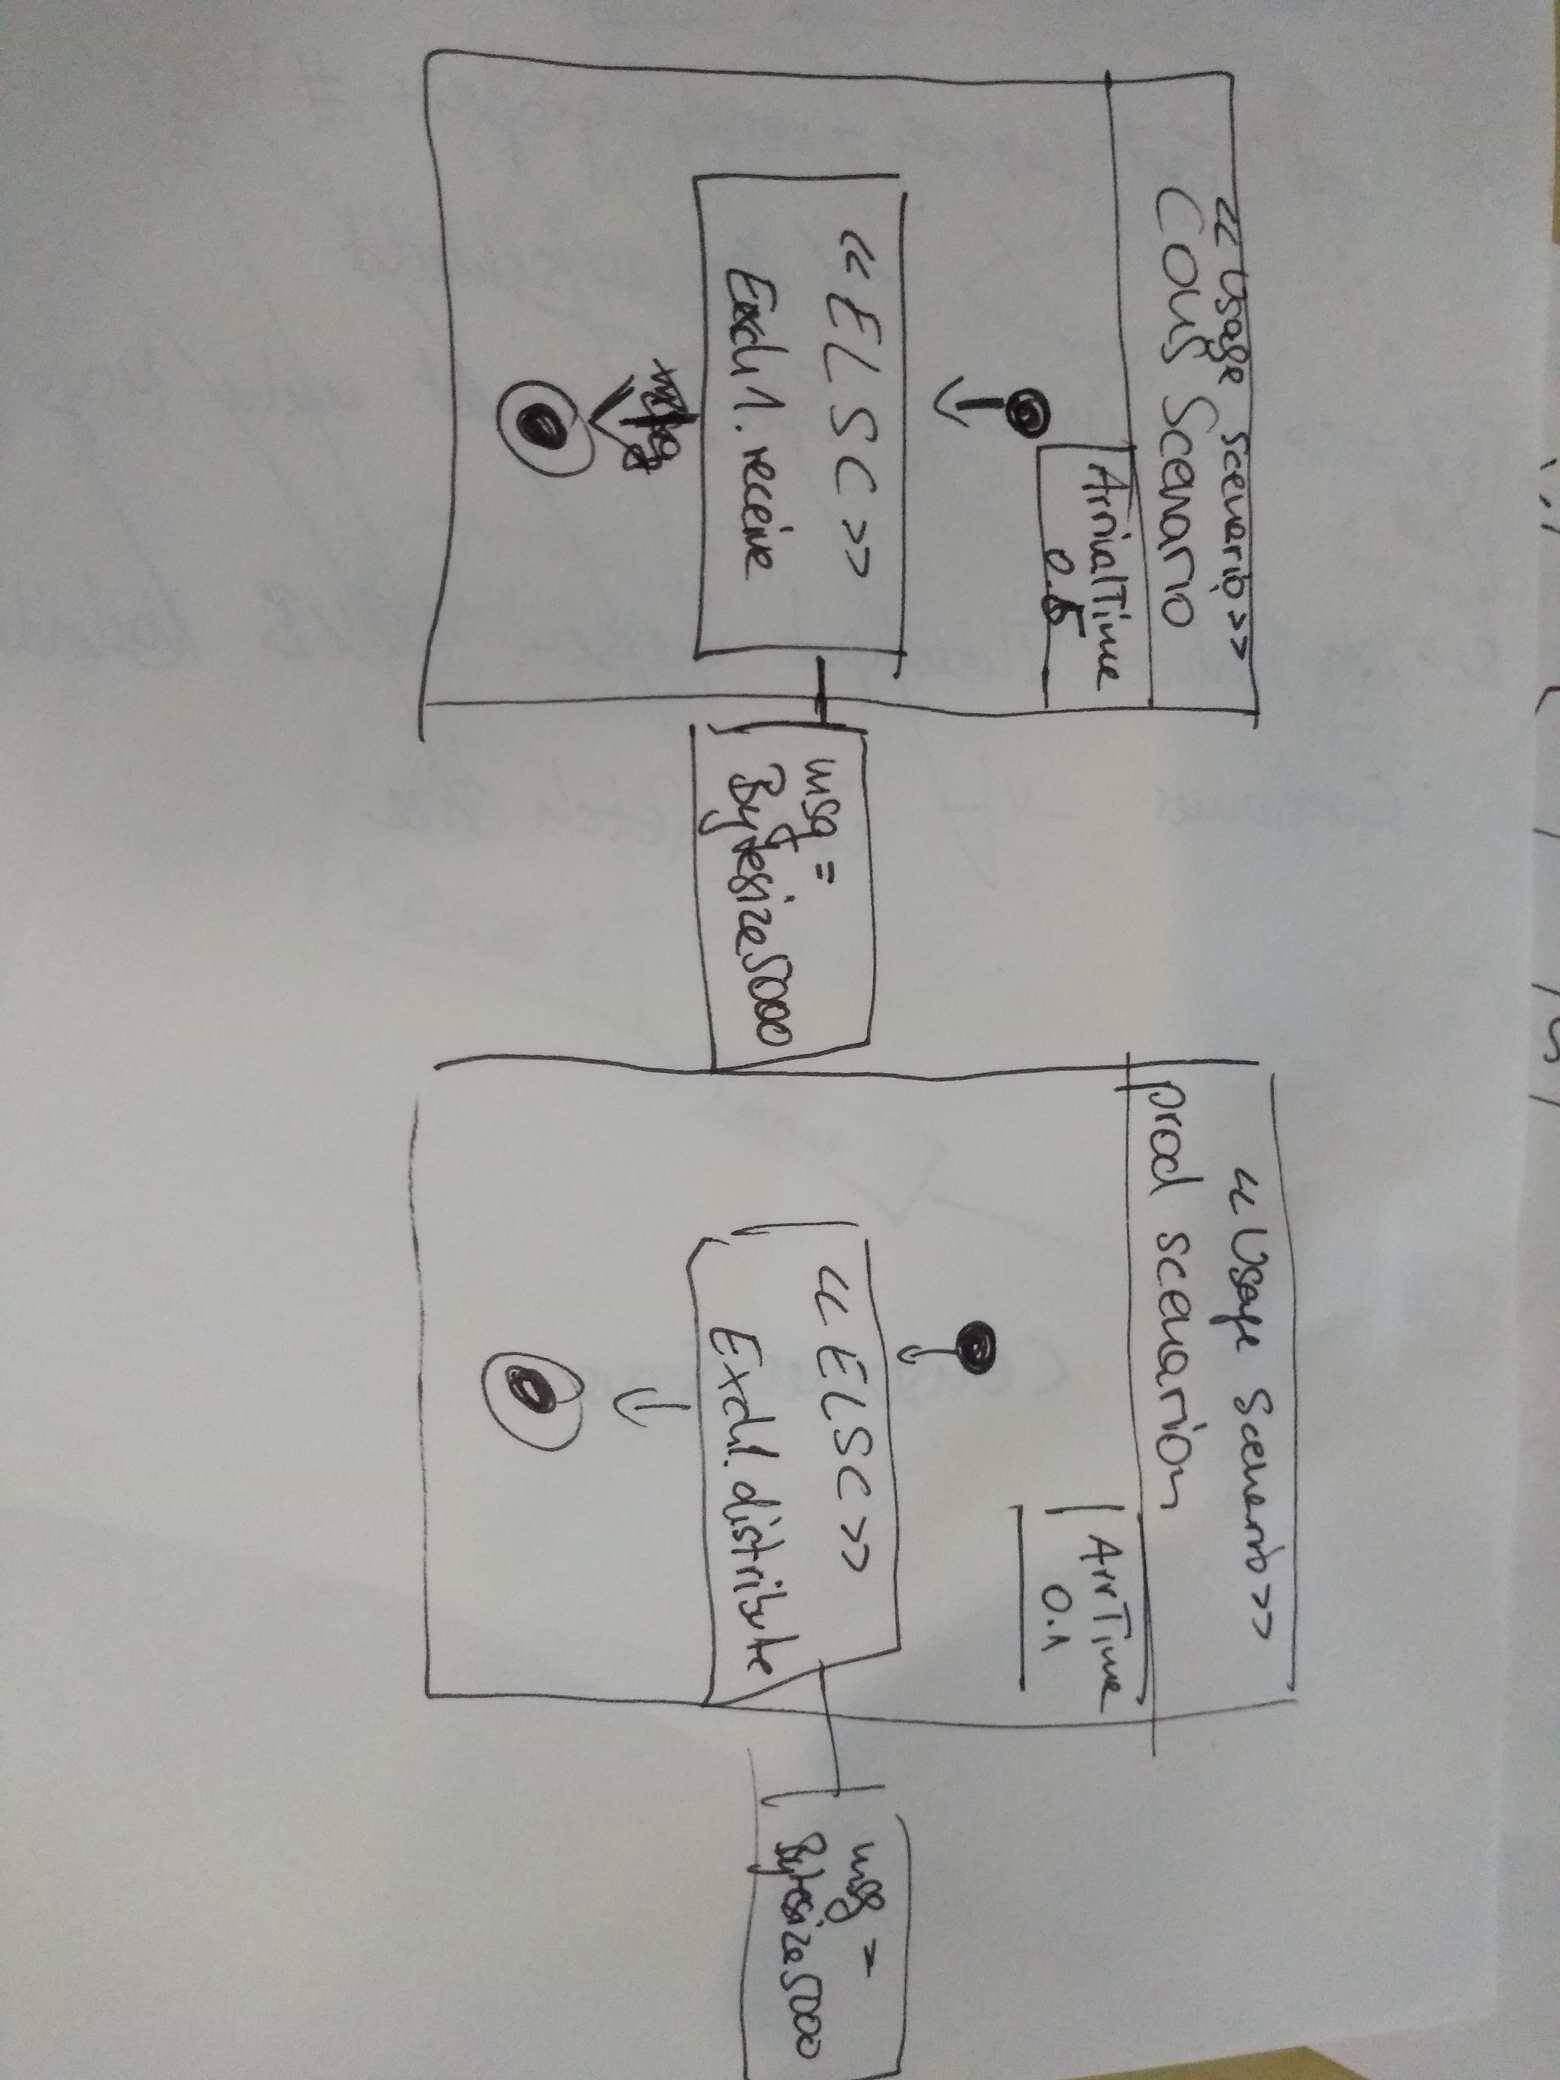
\includegraphics[width=1\textwidth]{images/modelling/usage.png}
  \caption{Nutzungsmodell einer MOM mit einem Sender und Empfänger}
  \label{img:mom_usage}
\end{figure}

\section{Modellkalibrierung}
\label{sec:rmqRd}
In \cite{palladio17} wird Modellkalibrierung als Anreicherung von Modellen mit quantitaitven Daten, wie Ressourcenbedarf. Je nachdem wie weit entwickelt das System ist, können diese Daten mithilfe von verschiedenen Techniken gewonnen werden. Mithilfe von Application-Performance-Monitoring wurde in \autoref{sec:rmqBenchmark} RMQ ausgemessen und die Ergbnisse dort beschrieben. Im Folgenden sollen die Ergebnisse interpretiert und benutzt werden um die Modelle zu kalibrieren.
%Das Ziel ist, dass der Benutzer keinen MOM spezifischen RD angeben muss. \\

In \autoref{oneMsgLatency} wurde die Latenz einer Nachricht mit verschiedenen Größen ausgemessen. Darin ist ein lineares Wachstum der Latenz mit ansteigen der Nachrichtengröße zu beobachten. Dies liegt die Vermutung nahe, dass diese beiden Variablen voneinander abhängen. Um diese Vermutung zu bestätigen wurde für die Variablen Latenz und Nachrichtengröße ihre Korellation berechnet. Dabei ist die Korrelation ein statistisches Maß, das den Grad der linearen Abhängigkeit zwischen zwei Variablen anzeigt, die im Paar auftreten. Ist diese Abhängigkeit hoch, liegt der Wert nahe eins. Liegt der Wert dagegen bei minus eins, ist die Abhängigkeit sehr gering. Die Korrelation der Variablen Latenz und Nachrichtengröße ist 0.9850627. Somit ist eine hohe lineare Abhängigkeit der Variablen gezeigt. Als nächstes soll mithilfe einer linearen Regressionsanalyse einen Ressourcenbedarf für das Modell definiert werden. Das Ziel einer linearen Regressionsanalyse ist es, eine lineare Beziehung zwischen einer Prädiktorvariable Y und der Reaktionsvariable X herzustellen, so dass der Wert von Y getschätzt werden kann, wenn nur der Wert des Prädiktoren X bekannt ist. Die Ergebnisse sind in \autoref{img:reganalysesummary} und die dabei entstandene Regressionsgerade in (abb) abgebildet. TODO was soll alles rein?
Daraus folgt ein Term der Form: Latenz = 1256.2782902 + (0.003299 * Nachrichtengröße). Dieser Term soll nun als Ressourcenbedarf einer Nachricht dienen, sobald diese aus der Warteschlange entnommen wird. 
\begin{figure}
\center
  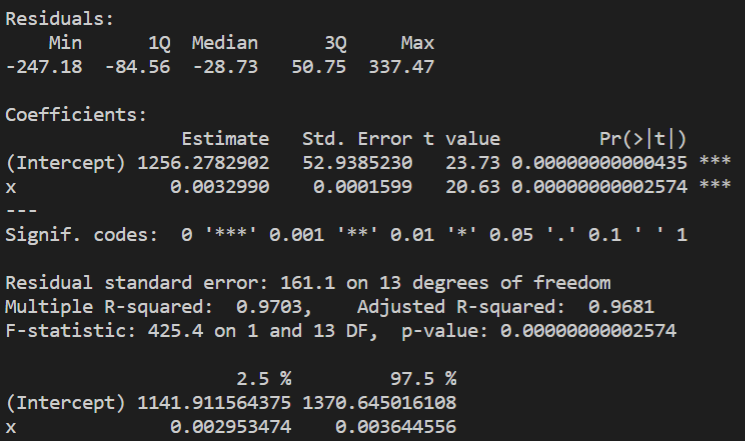
\includegraphics[width=1\textwidth]{images/modelling/reganalyse.png}
  \caption{Ergebniss der Regressionsanalyse}
  \label{img:reganalysesummary}
\end{figure}

\par

In \autoref{sec:maxthroughput} wurde gemessen, was die möglichen Datenmengen sind, die in dem System gesendet werden können. Dabei wurde eine Messung mit und ohne Empfänger durchgeführt. Der Maximalwert aus der Messung ohne Empfänger wird in die LinkingRessources zwischen dem MOM-RessourceContainer und dem Sender und der Maximalwert aus der Messung mit Empfänger wird in die LinkingRessources zwischen dem MOM-RessourceContainer und dem Empfänger jeweils als Throughput eingetragen. Sobald eine Nachricht über diese Verbindung gesendet wird, wird die Nachrichtengröße durch den Throughput geteilt und auf die Gesamtlatenz addiert. \par

Auch die Netzwerklatenz, die in \autoref{oneMsgLatency} ausgemessen wurde, hat einen Einfluss auf die Latenz einer Nachricht gehabt. Wenn diese in der Modellierung betrachtet werden soll, kann diese in die jeweiligen LinkingRessource als Netzwerklatenz eingetragen werden. Diese wird auf die Gesamtlatenz einer Nachricht addiert. \par

Neben der Standardkonfiguration wurde auch die Konfiguration für Lazy-Warteschlangen in \autoref{sec:rmqLazy} ausgemessen. Auch hier wurde wie oben beschrieben zunächst die Korrelation der beiden Variablen berechnet. Mit 0.9951195 ist diese ebenfalls sehr hoch. Die Ergebnisse der im Anschluss durchgeführten Regeressionsanalyse sind in  \autoref{img:reganalysesummarylazy} abgebildet. TODO was soll alles rein?
Daraus folgt ein Term der Form: Latenz = 1602.5021193 + (0.0049697 * Nachrichtengröße). Dieser Term soll nun als Ressourcenbedarf einer Nachricht dienen, sobald diese aus der Warteschlange entnommen wird, wenn Lazy-Warteschlangen betrachtet werden sollen.
\begin{figure}
\center
  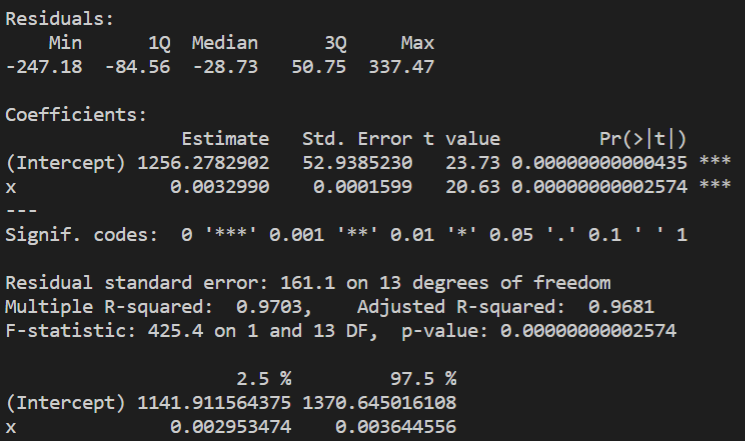
\includegraphics[width=1\textwidth]{images/modelling/reganalyse.png}
  \caption{Ergebniss der Regressionsanalyse}
  \label{img:reganalysesummarylazy}
\end{figure}

Die zuvor beschriebenen Modelle können nun mithilfe der hier vorgestellten quantitativen Daten angereichert werden um eine Performanzanalyse zu ermöglichen. Im nächsten Schritt soll eine konkrete Modellierung vorgestellt werden, die mit den hier vorgestellten Daten angereichert wird. 

%Somit ergibt sich f die Response Time folgendes ergeben: Response Time: ByteSize / Throughput + RD / CPU + Latency + HddRD/HDD \\
%RD an Aquire um Latenz abzubilden

%Als erstes sollte die Sende und Empfangsrate abgebildet werden. Beobachtet man (ref zu Messung verschiedene Senderaten) bemerkt man fuer die ersten Messungen, solange Warteschlange nicht allzu voll wird, einen linearen Anstieg der Latenz. Daraus laesst sich zunaechst folgender RD ableiten:






%Latenz: Unter Latenz versteht man im MOM Kontext, die Zeit, die eine einzelne Nachricht braucht um beim Consumer anzukommen. Da jede Nachricht einen Zeitstempel bekommt kann die Zeit gemessen werden, wenn sie aus der Warteschlange entnommen wurde.

%welche Effekte koennen wir so hoffentlich abbilden

\section{Untersuchung der MOM Modellierung}
In den Abschnitten zuvor wurde vorgestellt wie die Modellierung eines Systems aussehen soll, die eine MOM zum Nachrichtenaustausch verwendet. Im Folgenden wird eine konkrete Modellierung vorgestellt, die mit den quantitativen Daten aus \autoref{} angereichert wird. Anschließend wird eine Performanzanalyse auf der Modellierung ausgeführt. Die Ergebnisse werden anschließend mit den Messungen aus \autoref{sec:rmqBenchmark} verglichen.

\subsection{Anwendungszenario}
Im Folgenden betrachten wir das in \autoref{img:simulationscenario} abgebildete Szenario. Darin befindet sich eine Sender und eine Empfänger Komponente. Beide sind mit der Exchange Komponente verbunden. Der Exchange ist genau mit einer Warteschlange verbunden. Diese ist entweder mit dem RD für eine Nachricht ohne oder mit Lazy-Warteschlangen angereichert. Die Exchange und die Warteschlangen Komponente sind auf einem gemeinsamen ResourceContainer MOM bereitgestellt. Die Sender und Empfänger Komponente sind jeweils auf einem eigenen ResourceContainer bereitgestellt. Der MOM-RC ist jeweils mit dem Sender- und der Empfänger-RC mithilfe einer LinkingResource verbunden. Diese haben jeweils einen Wert für den Durchsatz und Latenz eingetragen, je nachdem welches Szenario betrachtet wird. Schließlich sind für den Sender und Empfänger jeweils ein UsageScenario spezifiziert. Darin sind die jeweiligen Ankunftszeiten und Nachrichtengrößen modelliert.
% Der Sender sendet pro Zeiteinheit und der Empfaenger empfaengt pro Zeiteinheit eine bestimmte Menge an verschieden Großen Nachrichten. 
\begin{figure}
\center
  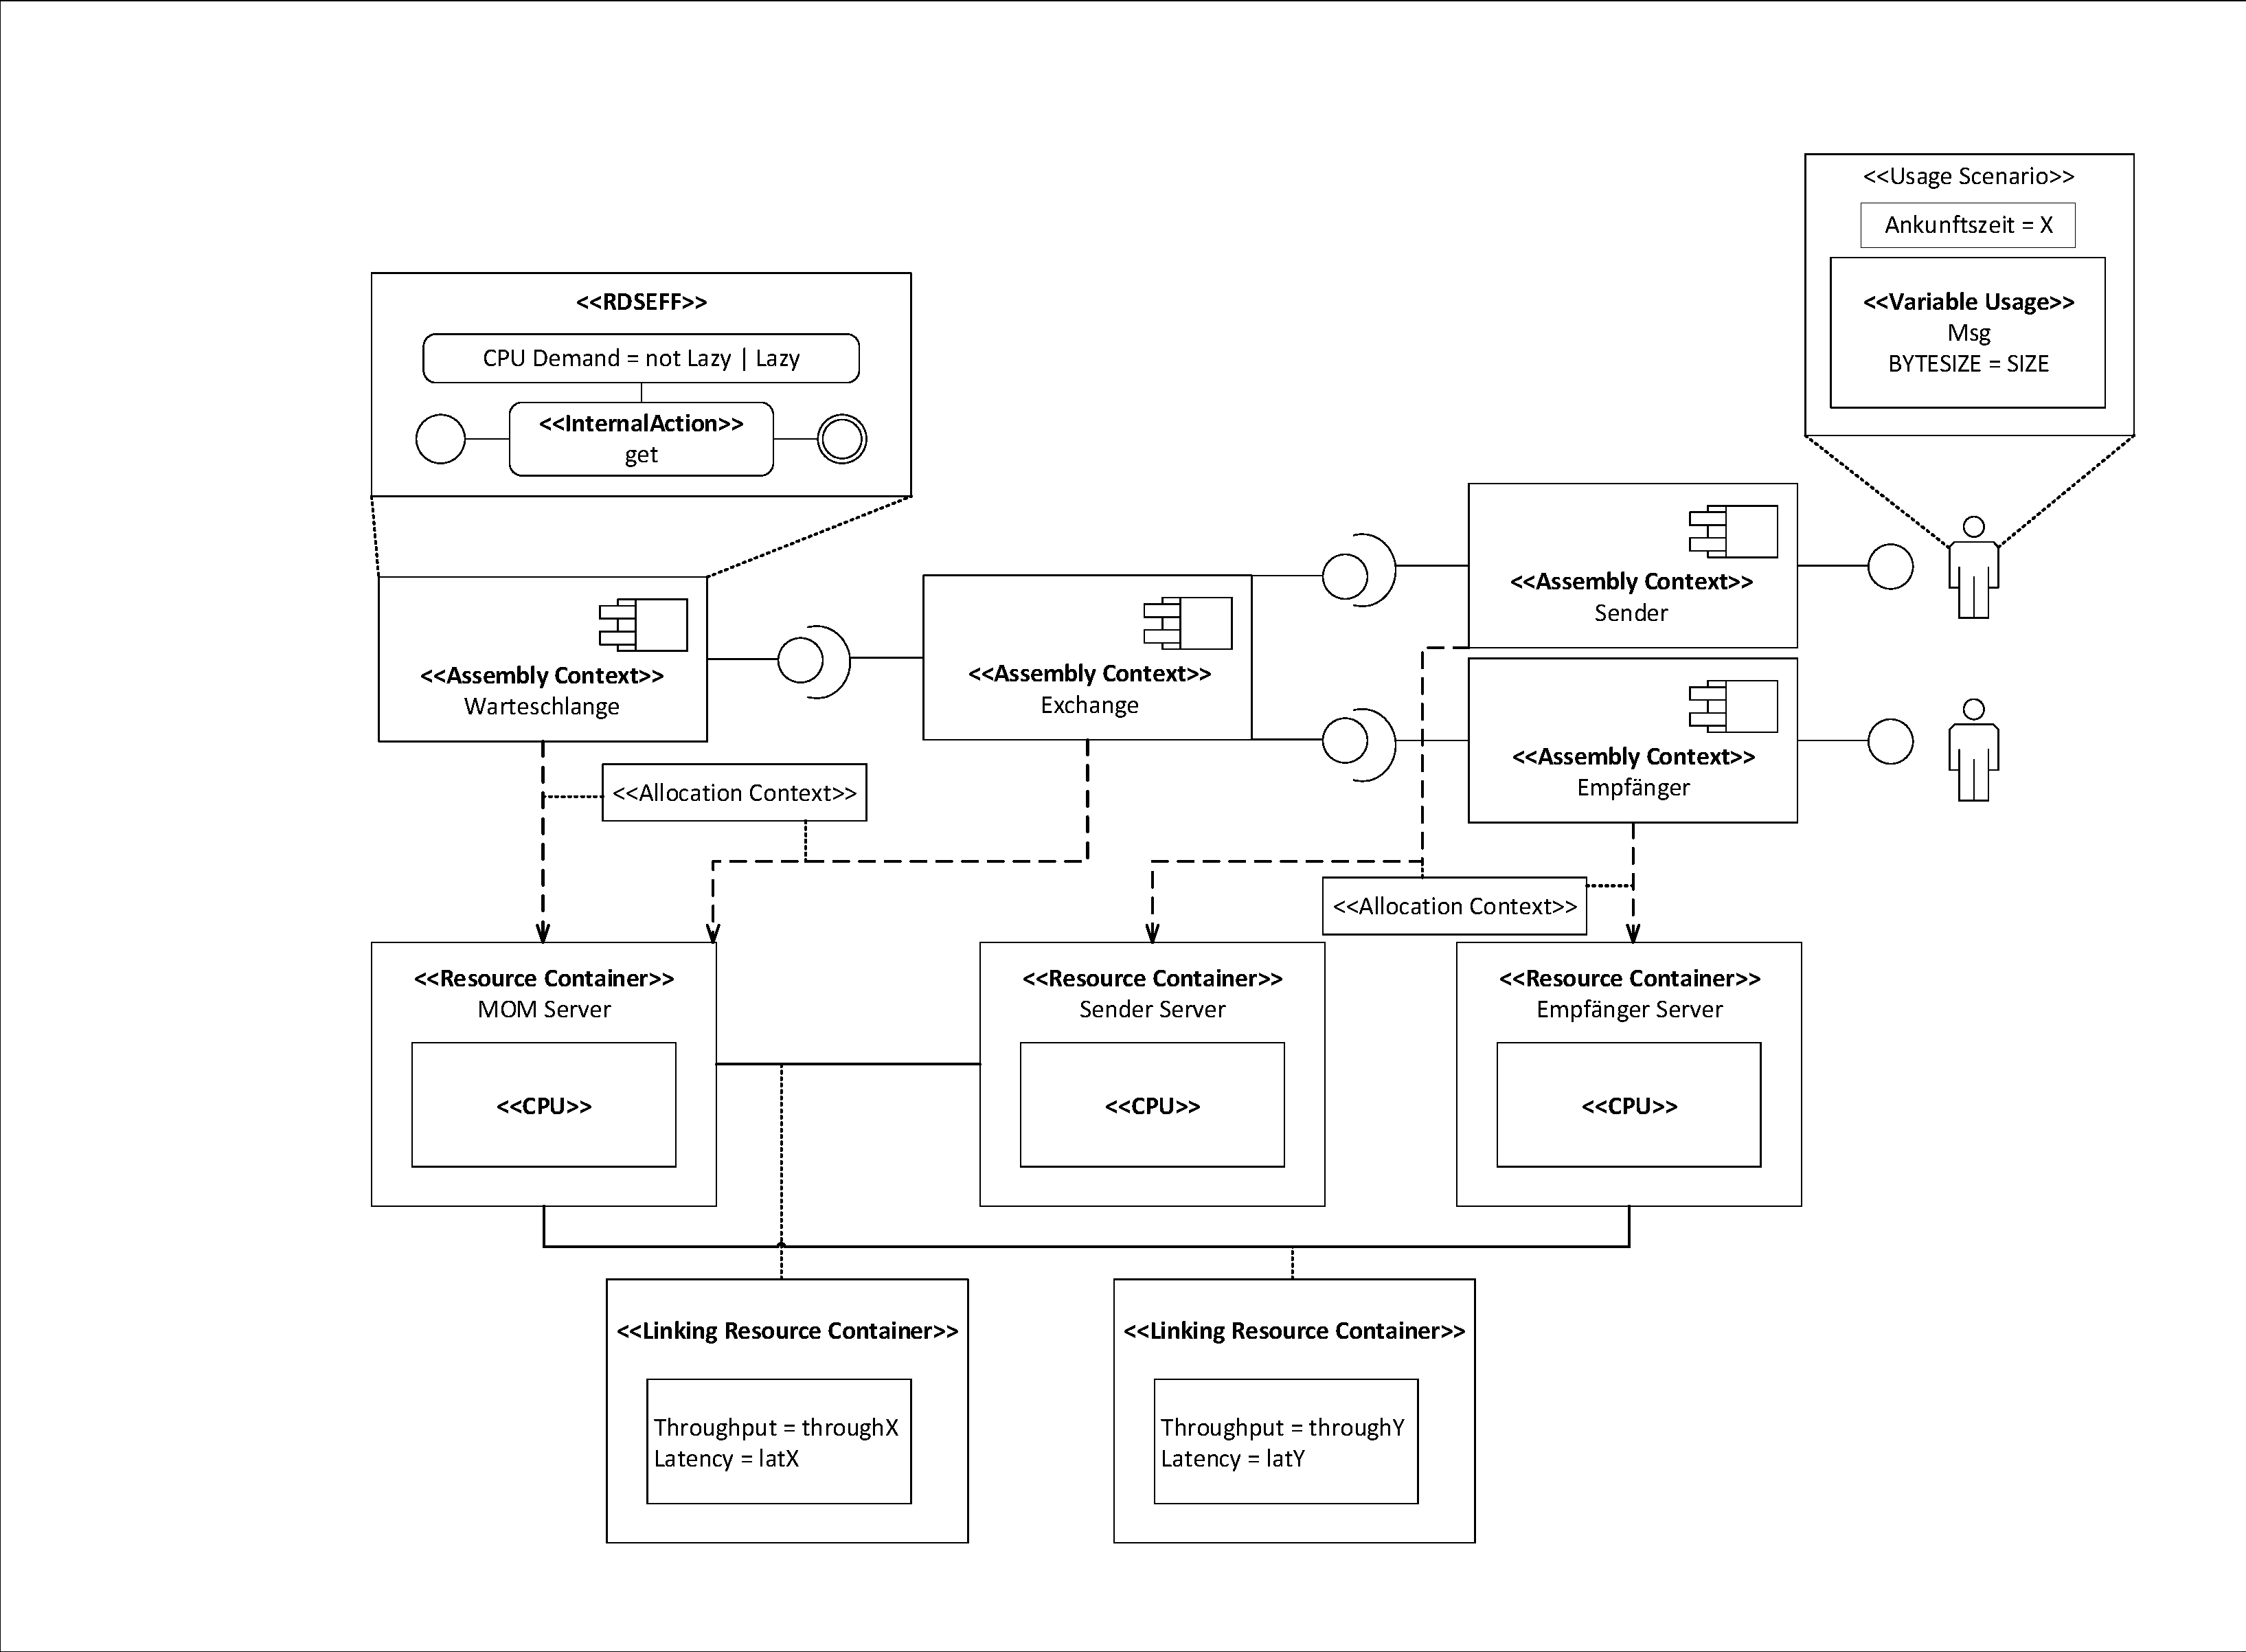
\includegraphics[width=1\textwidth]{images/modelSimulationResults/simulationScenario.pdf}
  \caption{Simulationsszenario }
  \label{img:simulationscenario}
\end{figure}
Im Folgenden wird diese Modellierung in einer Performanzanalyse eingesetzt.


\subsection{Performance-Analyse}
Die Palladio-Bench bietet eine Sammlung von Qualitätsanalysen mit Hauptfokus auf Performance an. Nachdem in den vergangen Abschnitten eine MOM Modellierung und ihre Kalibrierung beschrieben wurde, kann im nächsten Schritt eine Performance-Analyse ausgeführt werden. Dazu wird das Analysewerkzeug \textbf{SimuCom} verwendet, das verschiedene Performance Charakteristiken, darunter Antwortzeiten für Systeme und Komponenten, sowie die Auslastung einzelner Ressourcen berechnet. Im Folgenden werden die Ergebnisse der Performance-Analyse präsentiert und mit den Messungen aus \autoref{sec:rmqBenchmark} verglichen. Dazu wird für jede Simulation der Fehler zwischen dem gemessenen Wert und dem vom Modell vorhergesagten Wert berechnet. Dazu wird die Folgende Formel verwendet: \[ error\% = \frac{|prediction - measurement|}{measurement} * 100 \]. Für \textit{prediction} wird der Wert aus der Modell-Vorhersage eingesetzt. Für \textit{measurement} wird der jeweilige Median aus der Messungen eingesetzt.
\subsubsection{Simulation 1} 
\label{sec:rmqSimulation1}
In der ersten Simulation wird der Fall betrachtet, dass Sender und Empfänger die gleichen Ankunftszeiten haben. Die gesendete Nachrichten haben die Größen 100, 200, 300, 400, 500 und 1000 Kbyte. Verglichen wurde mit den Messungen aus \autoref{sec:oneMsgLatency}. Der Sender, Empfänger und der Broker befinden sich jeweils auf der selben Maschine. Betrachtet wurden der Füllstand der Warteschlange und die Latenz der Nachrichten. 
%B
Da die Ankunftszeiten der beiden Akteure gleich sind, bleibt die Warteschlange die ganze Zeit über Leer. Die Ergebnisse der Latenz einer Nachricht sind in \autoref{img:simulation1} abgebildet. Eingezeichnet sind dabei die Messpunkte der Messungen und die Ergebnisse der Simulation. In \autoref{tab:sim1} ist der Fehler für jede Größe angegeben. Dabei ist zu sehen, dass bei dieser Simulation der Fehler zwischen 19.98 \% und 30.67\% liegt.

\begin{figure}
\center
  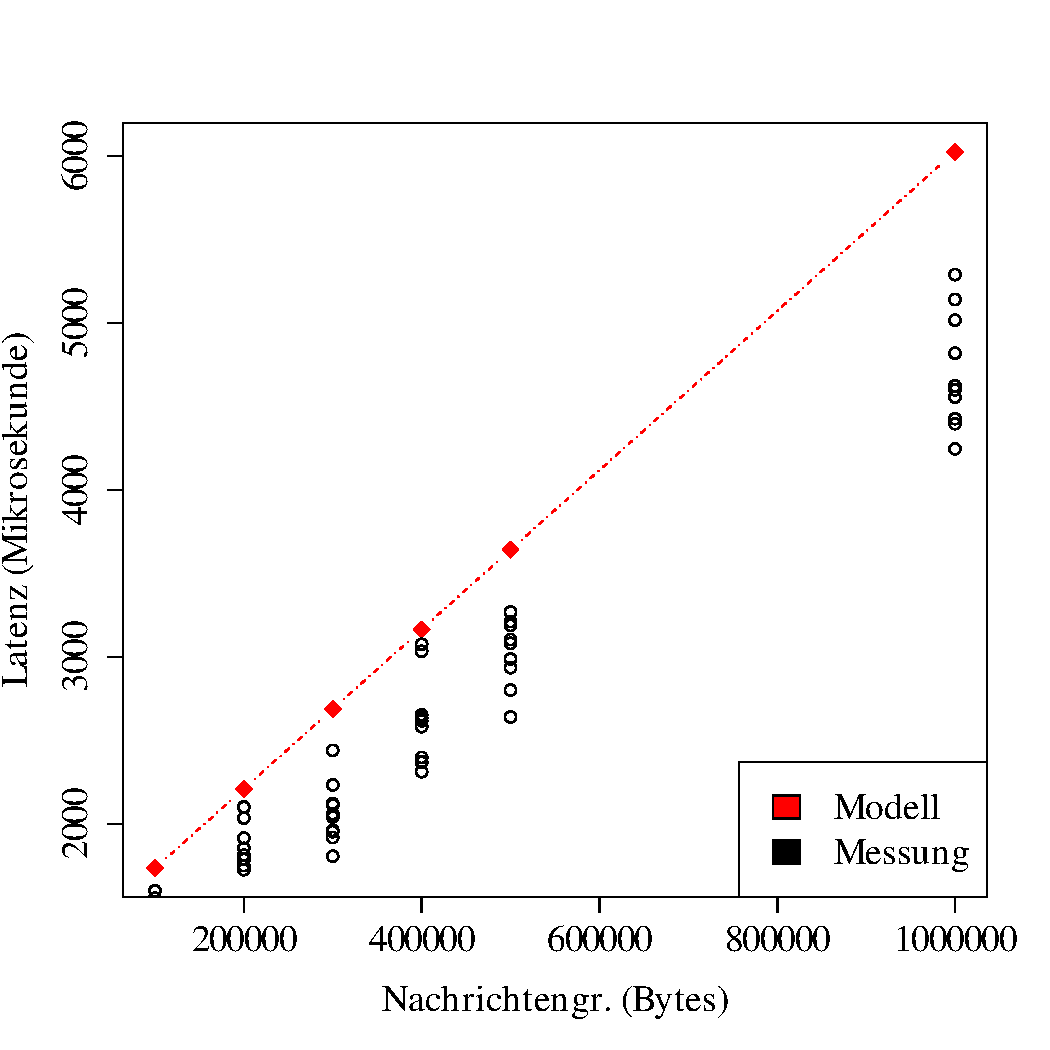
\includegraphics[width=0.5\textwidth]{images/modelSimulationResults/simulation1.pdf}
  \caption{Latenz einer Nachricht mit verschiedenen Groessen (Modell vs. Real System)}
  \label{img:simulation1}
\end{figure}

\begin{table}
  \begin{tabular}{| l | l | l | l |l | l | l |}
    \hline
    Nachrichtengröße (Kb) & 100 & 200 & 300 & 400 & 500 & 1000 \\ \hline
    Messung (\mu s) & 1339 & 1833 & 2050.5 & 2599.5 & 3035 & 4612\\ \hline
    Vorhersage (\mu s) & 1733.3 & 2210.3 & 2687.3 & 3164.3 & 3641.4 & 6026.5\\ \hline
    Fehler (\%) & 29.45 & 20.58 & 31.06 & 21.73 & 19.98 & 30.67\\ \hline
    
    \hline
      \end{tabular}
	\caption{\label{tab:sim1} Fehler in \% zwischen Messung und Modell Vorhersage für Simulation 1}
\end{table}





\subsubsection{Simulation 2} 
Diese Simulation betrachtet zusätzlich zu dem Fall aus Simulation 1 die Netzwerklatenz mit. Dazu sind Sender, Empfänger und Broker auf unterschiedlichen Maschinen. Die Nachrichten haben die größen 100, 200, 300, 400, 500 und 1000 Kbyte. Im Modell wurden für die LinkingRessources der Durchsatz und die Latenz, wie in \autoref{sec:rmqRd} beschrieben, für entfernte Broker angepasst. Die Messung mit der verglichen wurde ist in \autoref{sec:oneMsgLatency} beschrieben. Es wurden der Füllstand der Warteschlange und die Latenz der Nachrichten betrachtet. 
%B
Die Warteschlange bleibt über die Simulationsdauer leer, da die Ankunftszeiten der Sender und Empfänger gleich sind. Die Latenz der Nachrichten ist in \autoref{img:simulation2} abgebildet. Außerdem sind die Messpunkte aus der Messung eingetragen. In \autoref{tab:sim2} ist der Fehler für jede Größe angegeben. Der Fehler liegt zwischen 21.15\% und 33.43\%.
\begin{figure}
\center
  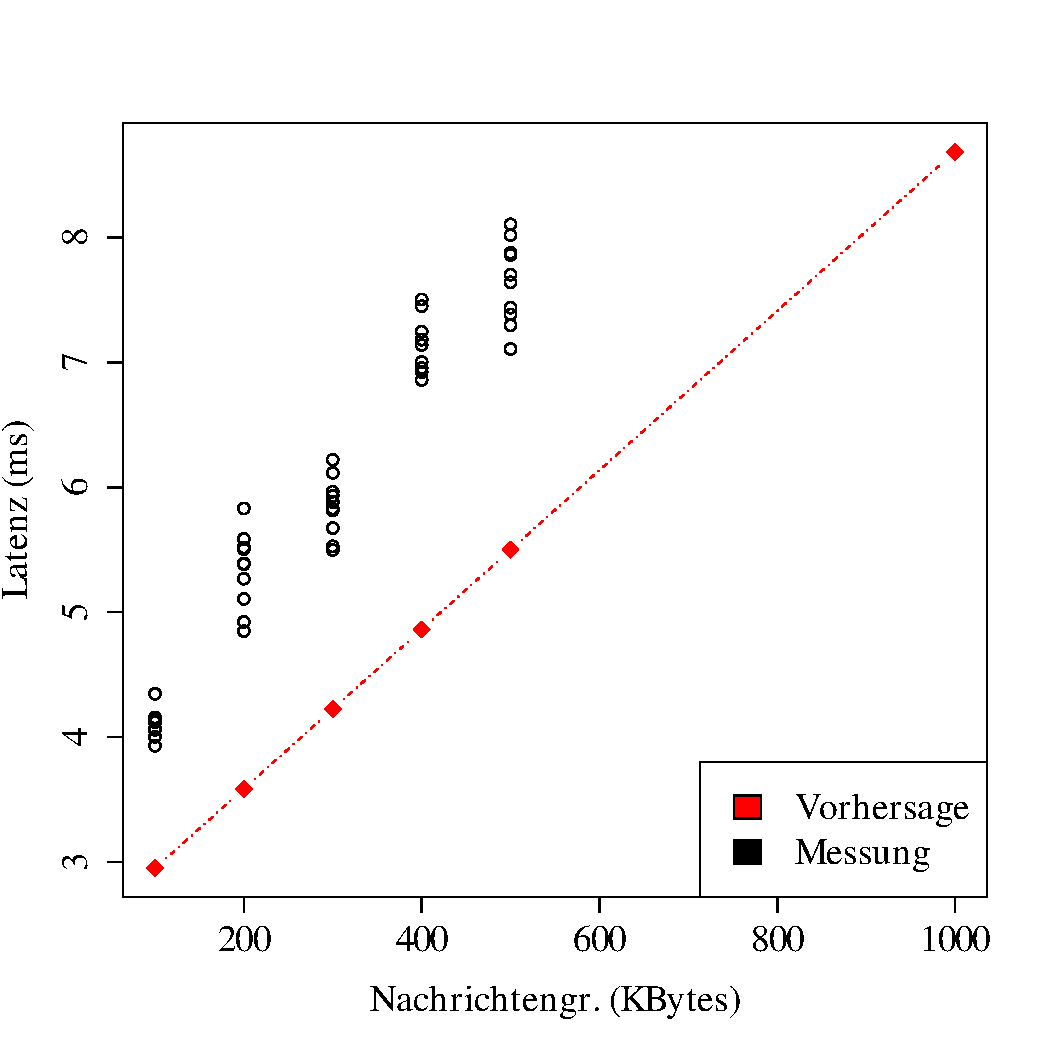
\includegraphics[width=0.5\textwidth]{images/modelSimulationResults/simulation2.pdf}
  \caption{Latenz einer Nachricht mit verschiedenen Groessen mit Netzwerklatenz (Modell vs. Real System)}
  \label{img:simulation2}
\end{figure}

\begin{table}
  \begin{tabular}{| l | l | l | l |l | l | l |}
    \hline
    Nachrichtengröße (Kb) & 100 & 200 & 300 & 400 & 500 & 1000 \\ \hline
    Messung (\mu s) & 4093 & 5387.5 & 5856.5 & 7161 & 7672.5 & 11019\\ \hline
    Vorhersage (\mu s) & 2948.71 & 3586.41 & 4224.12 & 4861.83 & 5499.53 & 8688.07\\ \hline
    Fehler (\%) & 27.96 & 33.43 & 27.87 & 32.11 & 28.32 & 21.15\\ \hline
    
    \hline
      \end{tabular}
	\caption{\label{tab:sim2} Fehler in \% zwischen Messung und Modell Vorhersage für Simulation 1}
\end{table}


\subsubsection{Simulation 3}
In dieser Simulation wird die Auswirkung der Ankunftszeiten auf das System geprüft. Verglichen wird mit der Messung aus \autoref{sec:queueGrowth}. Dabei ist die Ankunftszeit des Senders einmal pro Sekunde und die des Empfängers einmal alle zwei Sekunde. Der Füllstand der Warteschlange, sowie die Latenz der Nachrichten wird über die Zeit betrachtet.
%B
Die Ergebnisse sind in \autoref{img:simulation3} abgebildet. In \autoref{img:simulation3}a ist zu sehen, dass sich der Füllstand der Warteschlange bei Messung und Simulation gleich verhält und über die Zeit ansteigen, da jede Sekunde eine Nachricht in der Warteschlange unbearbeitet bleibt. In \autoref{img:simulation3}b sieht man außerdem die Auswirkungen auf die Latenz der einzelnen Nachrichten. Während bei der Messung die Latenz für die Nachrichten steigt, bleibt sie in der Modellierung unverändert. Dies liegt daran, dass die Latenz auch vom Füllstand der Warteschlange abhängt. In diesem Fall müsste der Füllstand bei der Berechnung der Latenz mit berücksichtigt werden. Dies ist mit SimuCom nicht möglich. 
\begin{figure}
\center
  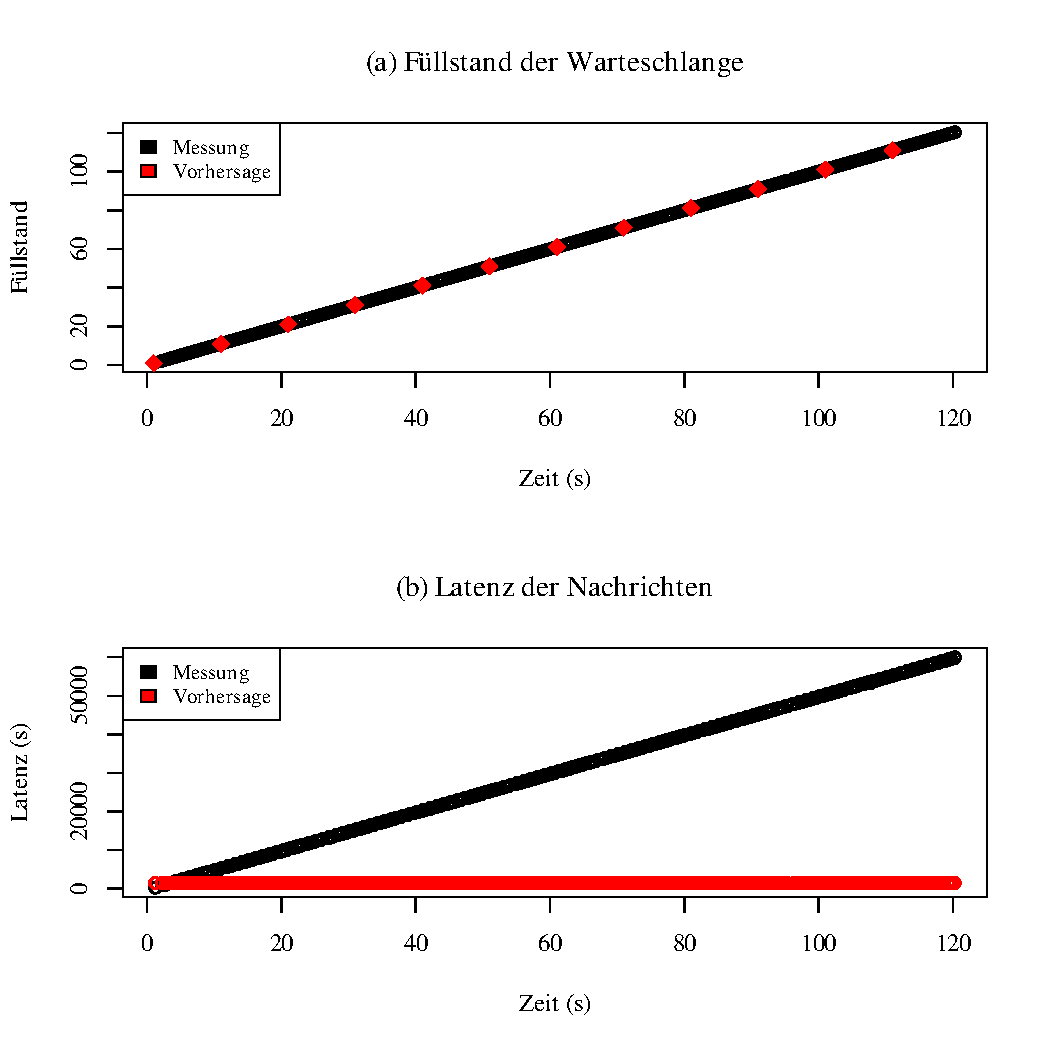
\includegraphics[width=0.5\textwidth]{images/modelSimulationResults/simulation3.pdf}
  \caption{Anwachsen der Warteschlange (Modell vs. Real System)}
  \label{img:simulation3}
\end{figure}

\subsubsection{Simulation 4}
Mit dieser Simulation soll die Auswirkung mehrerer Empfänger auf das System überpüft werden. Die Frage dabei ist, ob mehrere Empfänger eine Warteschlange gemeinsam abarbeiten können, wie in \autoref{sec:varyingConsumer} beschrieben. Obwohl in der Messung mit mehreren Empfängern, die Latenz nicht ganz an die Latenz eines Empfängers, der die Warteschlange alleine abarbeiten kann, herankommt, kann dieser Effekt aufgrund der minimalen Abweichung vernachlässigt werden. Im der folgenden Simulation ist die Ankunftszeit des Senders einmal pro Sekunde und die der beiden Empfänger jeweils einmal alle zwei Sekunden. Die Nachrichtengröße beträgt dabei, wie auch in der Messung, 10 KBytes. Betrachtet werden der Füllstand der Warteschlange und die Latenz der einzelnen Nachrichten. 
%B
Die Simulation zeigt, dass beide Empfänger die Warteschlange gemeinsam abarbeiten können. Der Fehler zwischen Messung und Vorhersage der Latenz liegt bei 4.4\%. 

\begin{figure}
\center
  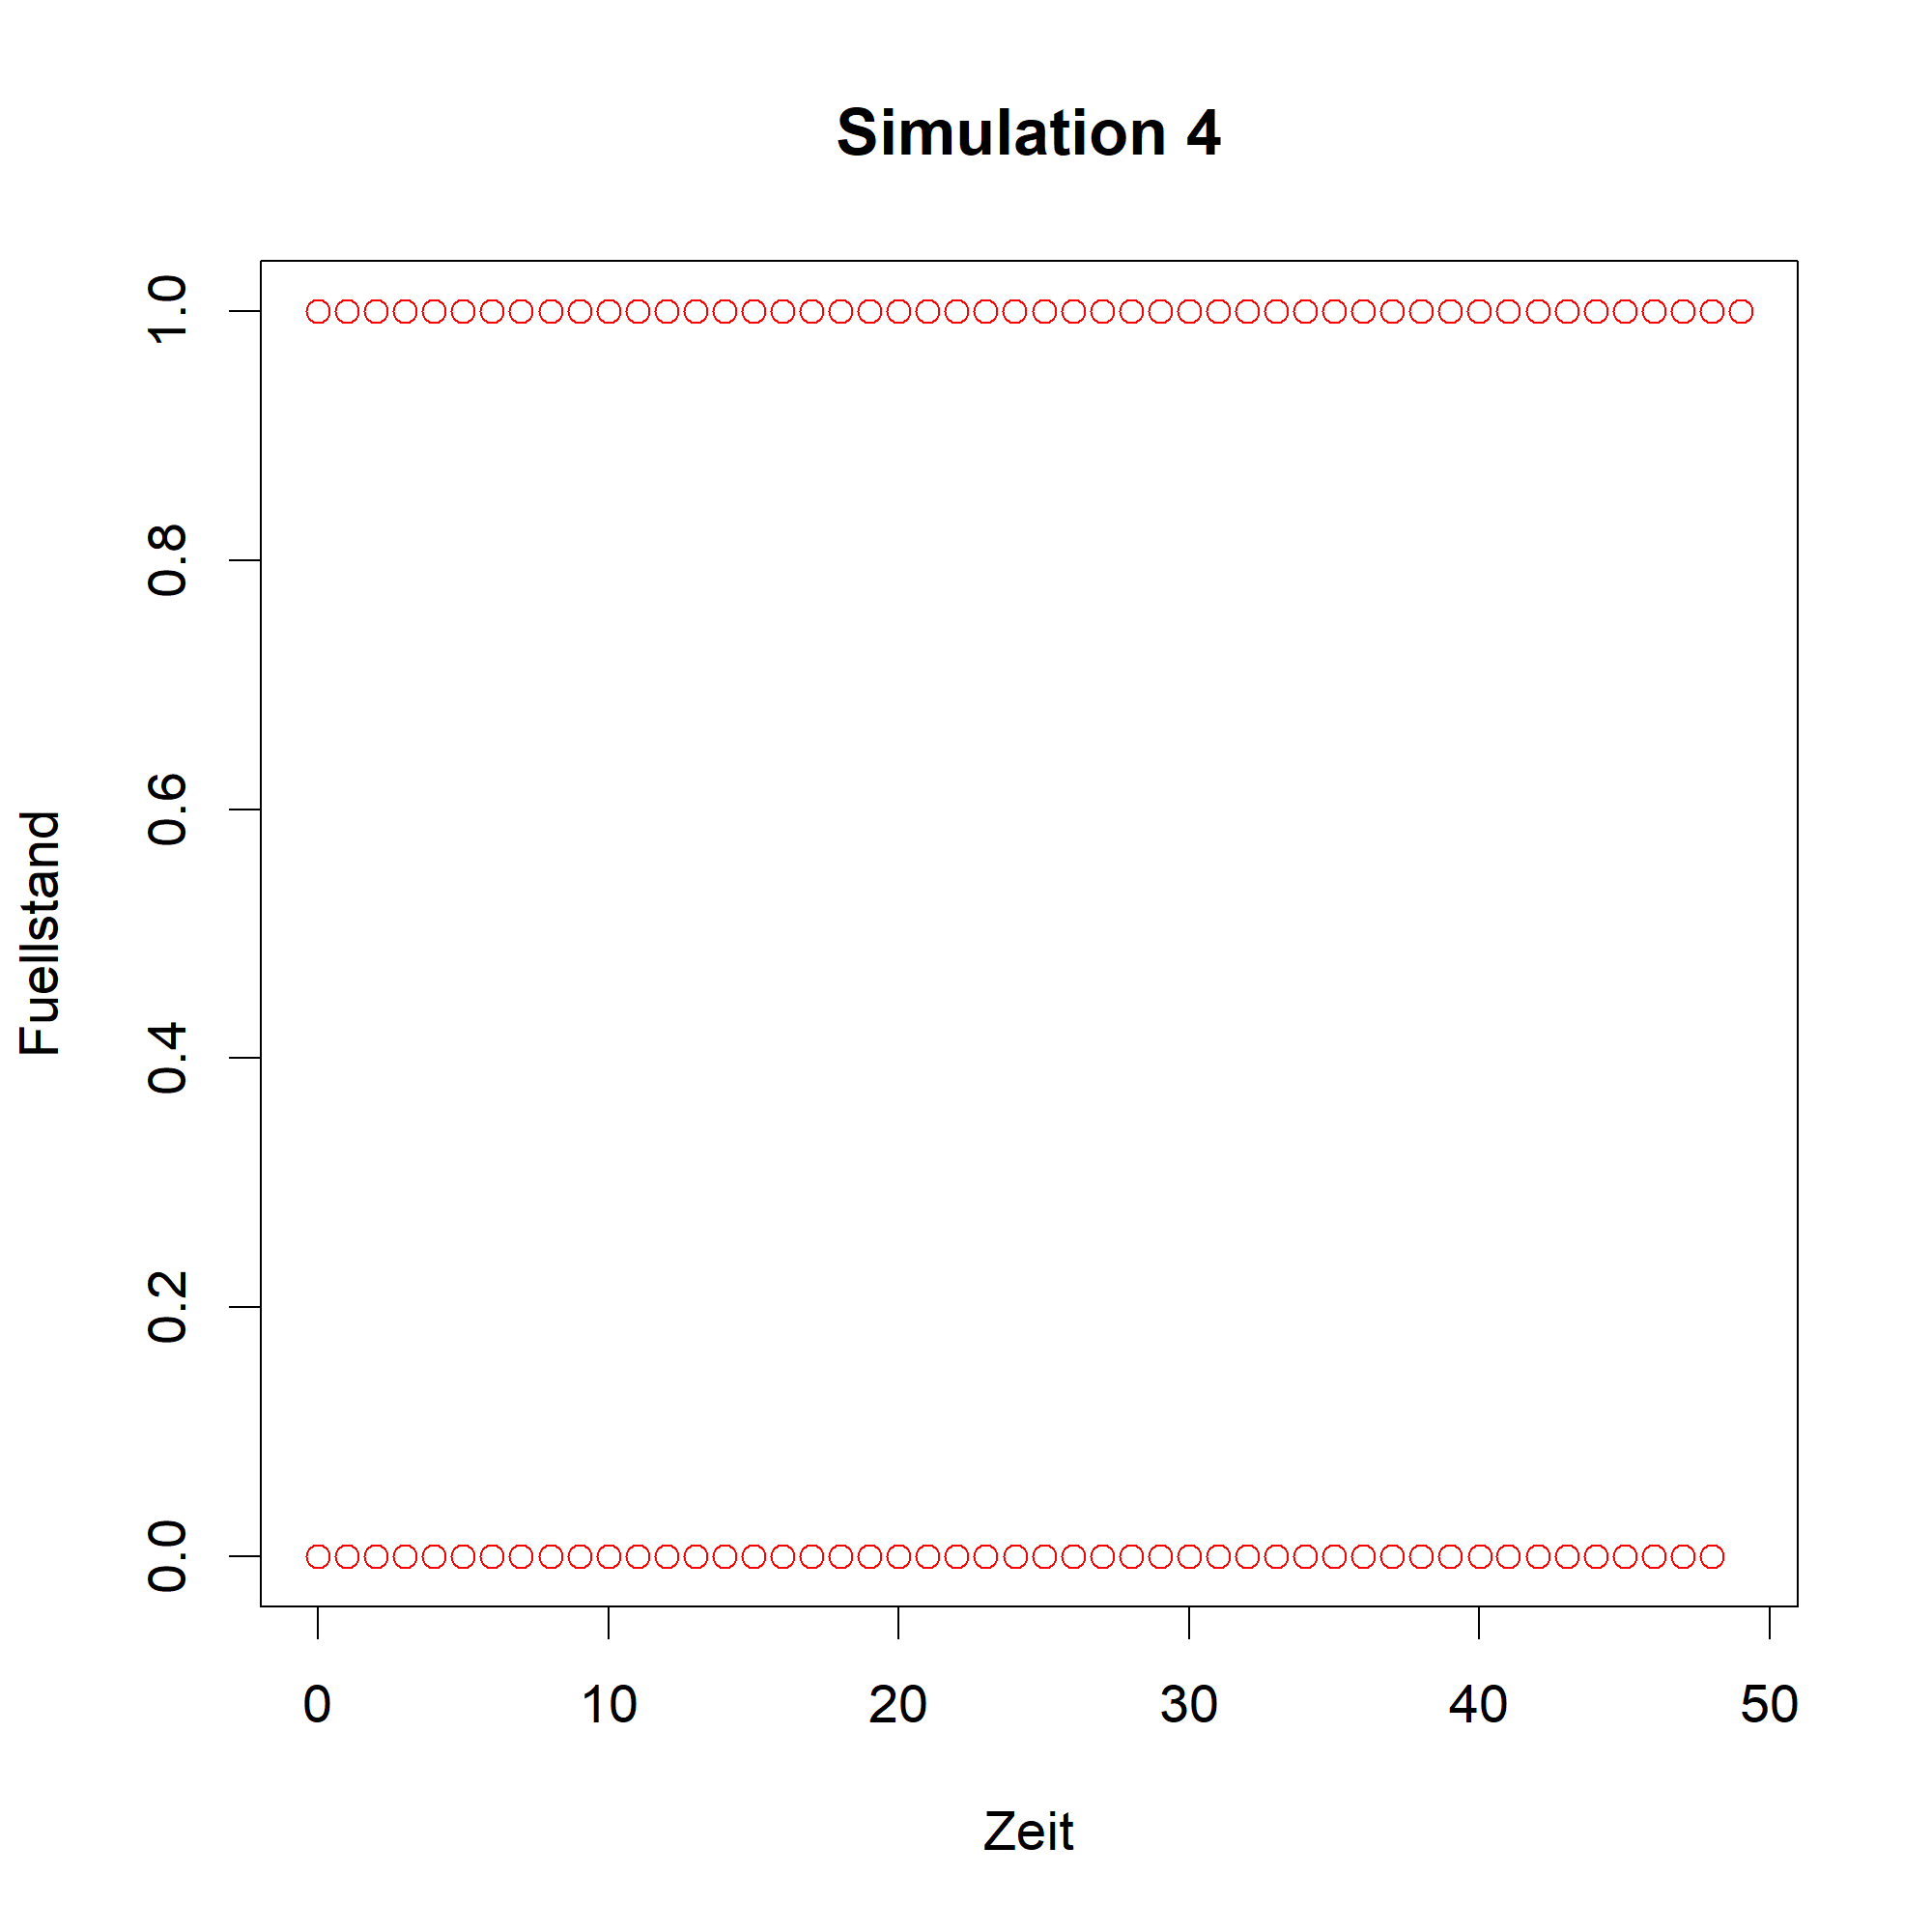
\includegraphics[width=0.5\textwidth]{images/modelSimulationResults/simulation4.png}
  \caption{Gemeinsames Abarbeiten einer Warteschlange durch zwei Empfaenger (Modell)}
  \label{img:simulation4}
\end{figure}

%Simulation 5: \\
%- Max Durchsatz \\
%- eine Nachricht mit max Bytesize schicken \\
%-> Response time sollte kontinuirlich ansteigen \\


\subsubsection{Simulation 5}
Schließlich betrachtet diese Simulation Lazy-Warteschlangen aus RMQ. Sender und Empfänger haben die gleiche Ankunftszeiten und kommen einmal pro Sekunde an. Die gesendete Nachrichten haben die Größe 100, 200, 300, 400, 500 und 1000 Kbyte. Der RD für eine Nachricht wurde im Modell angepasst. Dieser ist in \autoref{sec:rmqRd} beschrieben. Verglichen wurde mit der Messung aus \autoref{sec:rmqLazy}. Betrachtet wurde die Latenz der Nachrichten und der Füllstand der Warteschlange.
%B
Die Warteschlange bleibt aufgrunde der gleichen Ankuftszeiten gleich. In \autoref{img:simulation6} sind die Ergebnisse bezüglich der Latenz abgebildet. Neben den Vorhersagepunkten aus dieser Simulation und den Messpunkte aus der Messung mit Lazy-Warteschlangen, sind die Vorhersagepunkte aus \autoref{sec:rmqSimulation1} eingetragen. In \autoref{tab:sim5} sind die Fehler abgebildet. Dabei wird neben dem Fehler zur Messung mit Lazy-Warteschlangen und der Vorhersage mit Lazy-Warteschlangen auch der Fehler zwischen der Messung mit Lazy-Warteschlangen und der Vorhersage aus \autoref{sec:rmqSimulation1} berechnet. Dabei ist zunächst zu sehen, dass der Fehler zwischen der Messung und der Vorhersage mit Lazy-Warteschlangen zwischen 10.14\% und 22.12\% liegt. Der Fehler zwischen der Messung mit Lazy-Warteschlangen und der Vorhersage aus \autoref{sec:rmqSimulation1} liegt zwischen 7.38\% und 15.78\% und ist somit besser. TODO begründung warum dieser denoch nicht verwendet werden soll oder weglassen?.
\begin{figure}
\center
  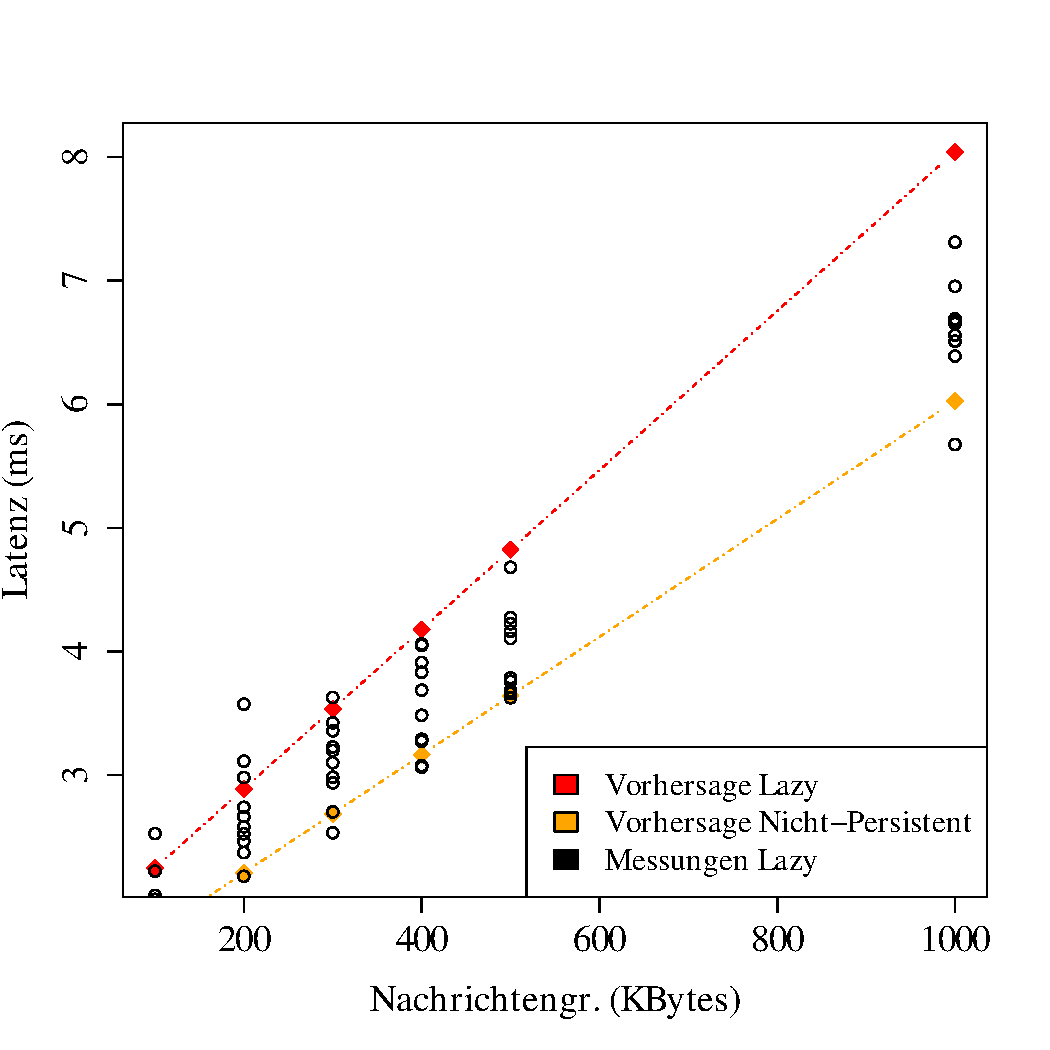
\includegraphics[width=0.5\textwidth]{images/modelSimulationResults/simulation6.pdf}
  \caption{Latenz einer Nachricht mit verschiedenen Groessen bei Lazy Warteschlangen (Modell vs. Real System)}
  \label{img:simulation6}
\end{figure}

\begin{table}
  \begin{tabular}{| l | l | l | l |l | l | l |}
    \hline
    Nachrichtengröße (Kb) & 100 & 200 & 300 & 400 & 500 & 1000 \\ \hline
    Messung (\mu s) & 1871.5 & 2624.5 & 3150 & 3586.5 & 3946.5 & 6663.5\\ \hline
    Vorhersage (\mu s) & 2246.59 & 2890.68 & 3534.77 & 4178.85 & 4822.94 & 8043.38\\ \hline
    Fehler (\%) & 20.04 & 10.14 & 12.21 & 16.52 & 22.21 & 20.71\\ \hline
    Fehler (\%) (ohne Lazy) & 7.38 & 15.78 & 14.69 & 11.77 & 7.73 & 9.56\\ \hline
    
    
    \hline
      \end{tabular}
	\caption{\label{tab:sim5} Fehler in \% zwischen Messung und Modell Vorhersage für Simulation 1}
\end{table}


\section{Grenzen}
Dieser Ansatz ermöglicht es jedoch nicht einzelne Nachrichten durch das System zu verfolgen\\

welche Moeglichkeiten gibt es? Dominiks Queue Modell. Direkt drauf verweisen, oder eine/diese Idee beschreiben.\\
%Queue Fuellstand ist unbekannt \\

%Nachdem eine MOM in das Experimentsystem eingebaut wurde, soll sie im Anschluss in Palladio modelliert werden. Wie bereits erwähnt existiert eine Palladio Modellierung des Experimentsystem, auf der aufgebaut werden kann. Bei der Modellierung der MOM soll zunächst die Standardkonfiguration und in späteren Iterationen Parametrisierbarkeit modelliert werden. Dazu soll zunächst versucht werden die MOM mithilfe vorhandener PCM Elementen zu modellieren und Unzugänglichkeiten zu identifizieren. Die Idee ist, mithilfe von Architecture-Templates \cite{architcturetemplate} diese Unzugänglichkeiten zu beseitigen. Dabei handelt es sich um wiederverwendbare Muster, die auf Palladio-Modelle angewendet werden können. Beispielsweise kann anstelle der manuellen Modellierung eines Lastverteilers auch das Architectural-Template für Lastverteiler verwendet werden. %Da diese Anwendung nur aus wenigen kleinen Schritten besteht, können Architekten viel Modellierungsaufwand einsparen.


%(-- RabitMQ Config:)\\% https://www.rabbitmq.com/configure.html\\
%(-- Kafka Config:)\\ %https://kafka.apache.org/documentation/#brokerconfigs 

